% Autor: Leonhard Segger, Alexander Neuwirth
% Datum: 2017-10-30
\documentclass[
	% Papierformat
	a4paper,
	% Schriftgröße (beliebige Größen mit „fontsize=Xpt“)
	12pt,
	% Schreibt die Papiergröße korrekt ins Ausgabedokument
	pagesize,
	% Sprache für z.B. Babel
	ngerman
]{scrartcl}

% Achtung: Die Reihenfolge der Pakete kann (leider) wichtig sein!
% Insbesondere sollten (so wie hier) babel, fontenc und inputenc (in dieser
% Reihenfolge) als Erstes und hyperref und cleveref (Reihenfolge auch hier
% beachten) als Letztes geladen werden!

\usepackage{tikz}
\usetikzlibrary{calc,patterns,angles,quotes} % loads some tikz extensions\usepackage{tikz}
\usetikzlibrary{babel}

% Silbentrennung etc.; Sprache wird durch Option bei \documentclass festgelegt
\usepackage{babel}
% Verwendung der Zeichentabelle T1 (Sonderzeichen etc.)
\usepackage[T1]{fontenc}
% Legt die Zeichenkodierung der Eingabedatei fest, z.B. UTF-8
\usepackage[utf8]{inputenc}
% Schriftart
\usepackage{lmodern}
% Zusätzliche Sonderzeichen
\usepackage{textcomp}

% Mathepaket (intlimits: Grenzen über/unter Integralzeichen)
\usepackage[intlimits]{amsmath}
% Ermöglicht die Nutzung von \SI{Zahl}{Einheit} u.a.
\usepackage{siunitx}
% Zum flexiblen Einbinden von Grafiken (\includegraphics)
\usepackage{graphicx}
% Abbildungen im Fließtext
\usepackage{wrapfig}
% Abbildungen nebeneinander (subfigure, subtable)
\usepackage{subcaption}
% Funktionen für Anführungszeichen
\usepackage{csquotes}
\MakeOuterQuote{"}
% Zitieren, Bibliografie
\usepackage[sorting=none]{biblatex}


% Zur Darstellung von Webadressen
\usepackage{url}
%chemische Formeln
\usepackage[version=4]{mhchem}
% siunitx: Deutsche Ausgabe, Messfehler getrennt mit ± ausgeben
\usepackage{floatrow}
\floatsetup[table]{capposition=top}
\usepackage{float}
% Verlinkt Textstellen im PDF-Dokument
\usepackage[unicode]{hyperref}
% "Schlaue" Referenzen (nach hyperref laden!)
\usepackage{cleveref}
\sisetup{
	locale=DE,
	separate-uncertainty
}
\bibliography{BA-C-04_V01_13-05-2019_References}

\begin{document}

	\begin{titlepage}
		\centering
		{\scshape\LARGE Versuchsbericht zu \par}
		\vspace{1cm}
		{\scshape\huge V01 - NaI- und Ge-Detektor \par}
		\vspace{2.5cm}
		{\LARGE Gruppe BA-C-04 \par}
		\vspace{0.5cm}

		{\large Alexander Neuwirth (E-Mail: a\_neuw01@wwu.de) \par}
		{\large Leonhard Segger (E-Mail: l\_segg03@uni-muenster.de) \par}
		\vfill

		durchgeführt am 13.05.2019\par
		betreut von\par
		{\large Axel Buß}

		\vfill

		{\large \today\par}
	\end{titlepage}
	\tableofcontents
	\newpage

	\section{Kurzfassung}
	% Hypothese	und deren Ergebnis, wenn Hypothese ist, dass nur Theorie erfüllt, sagen: Erwartung: Theorie aus einführung (mit reflink) erfüllt
	% Ergebnisse, auch Zahlen, mindestens wenn's halbwegs Sinn ergibt
	% Was wurde gemacht
	% manche leute wollen Passiv oder "man", manche nicht

  \section{Theorie}
	% wdh. Texte
	% wdh. Besprechung

	\begin{figure}[H]
			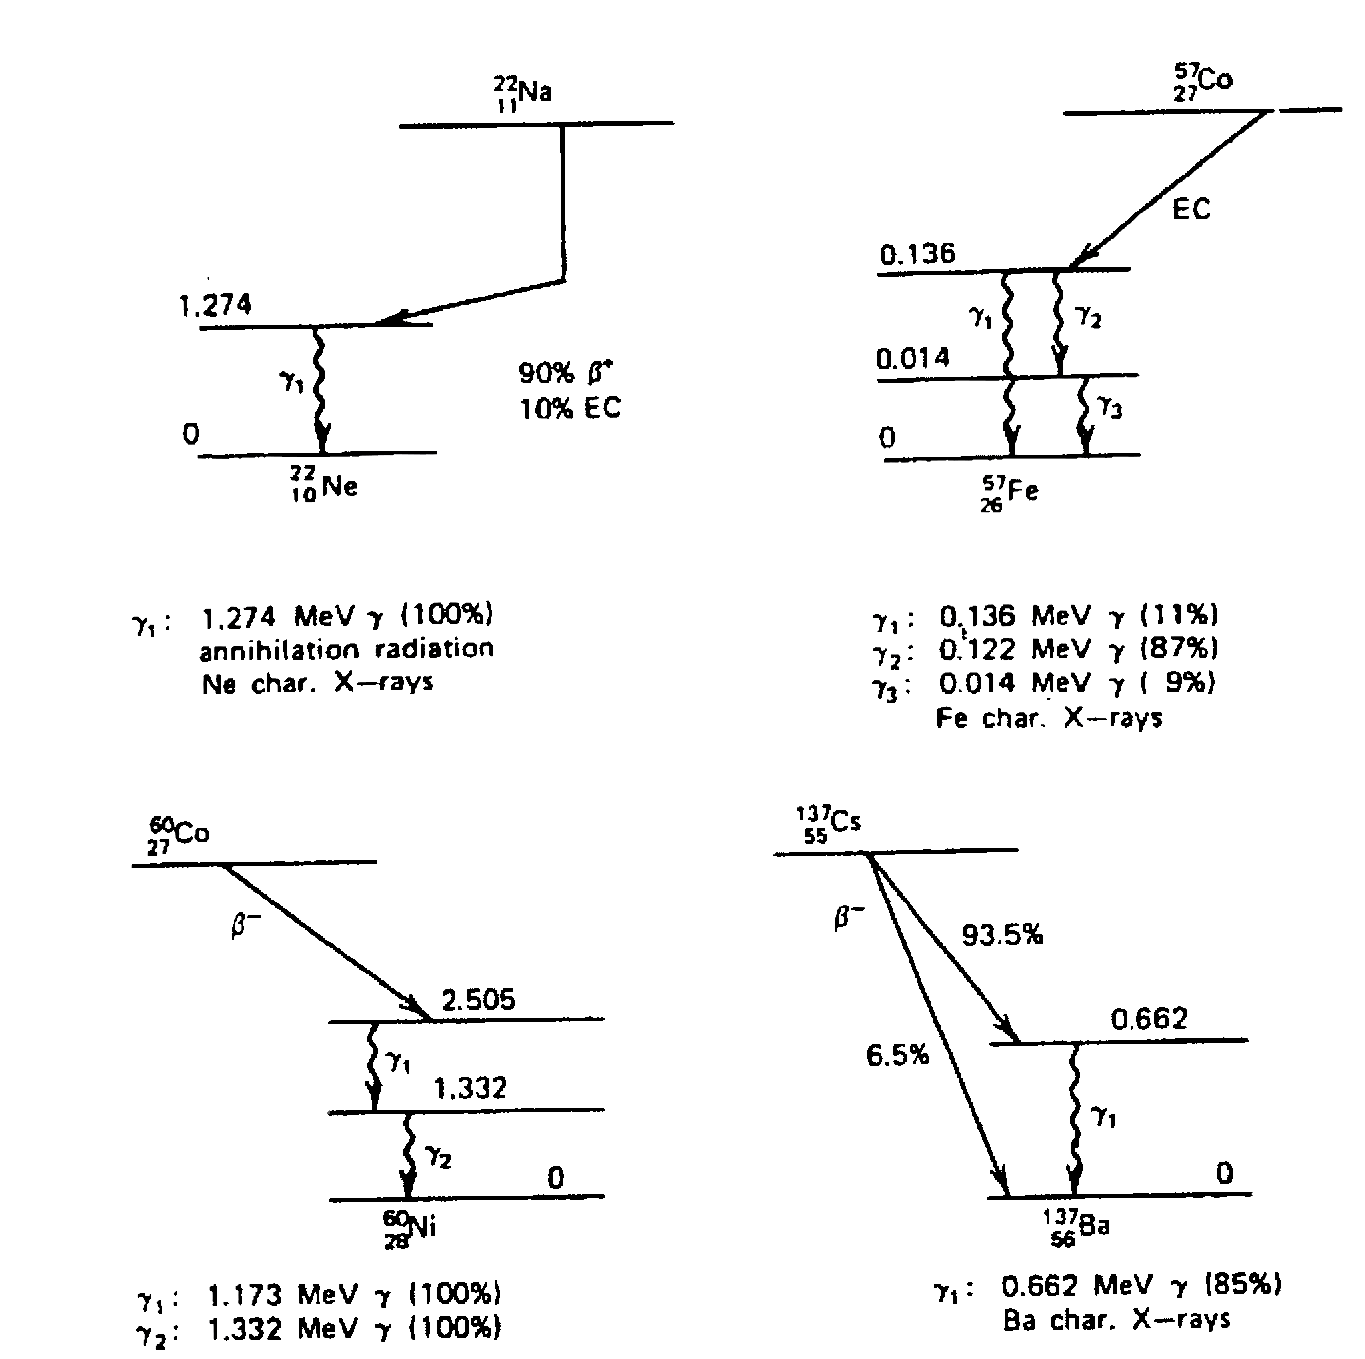
\includegraphics[width= 1 \linewidth]{charts/Zerfallsschemata}
			\caption{
				Zerfallsschemata der relevanten Zerfälle. %TODO
				\cite{Anleitung}
			}
			\label{fig_zerfallsschemata}
	\end{figure}

	\section{Methoden}
	% Bilder von der Website klauen
	% einer will Präsens

	\section{Ergebnisse und Diskussion}
	%TODO Unsicherheiten


	\subsection{Beobachtung und Datenanalyse}
	% Allgemeine Beobachtungen
	% Einflüsse von veränderten Parametern auf Messung

	\subsubsection{Unsicherheiten}
	Alle Unsicherheiten werden nach GUM bestimmt und berechnet.
	Für diese Berechnungen wurde die Python Bibliothek \enquote{uncertainties} herangezogen, welche den Richtlinien des GUM folgt.
	Die Fits verwenden die Methode der kleinsten Quadrate, außer wenn anders angegeben.
	Die Unsicherheit der gemessenen Ereignisse $N$ ist durch $\sqrt{N}$ gemäß Poisson-Verteilung gegeben.
	\subsubsection{Modell}
	Die aufgenommenen Spektren der $^{22}$Na-Probe sind in \cref{fg_Na_ch} abgebildet.
	Es wurde bei jeder Messung die ersten 95 Kanäle vernachlässigt, da all diese nahe Null Ereignisse liefern und die Erstellung ein physikalischen Modells des Spektrums im Randbereich unmöglich machen. %TODO schönerer Satz wäre schöner
	Das Modell wurde in \enquote{Fityk} aus Gaußkurven zusammengesetzt.
	\begin{figure}[H]
		\centering
		\begin{subfigure}[c]{\textwidth}
			\centering
			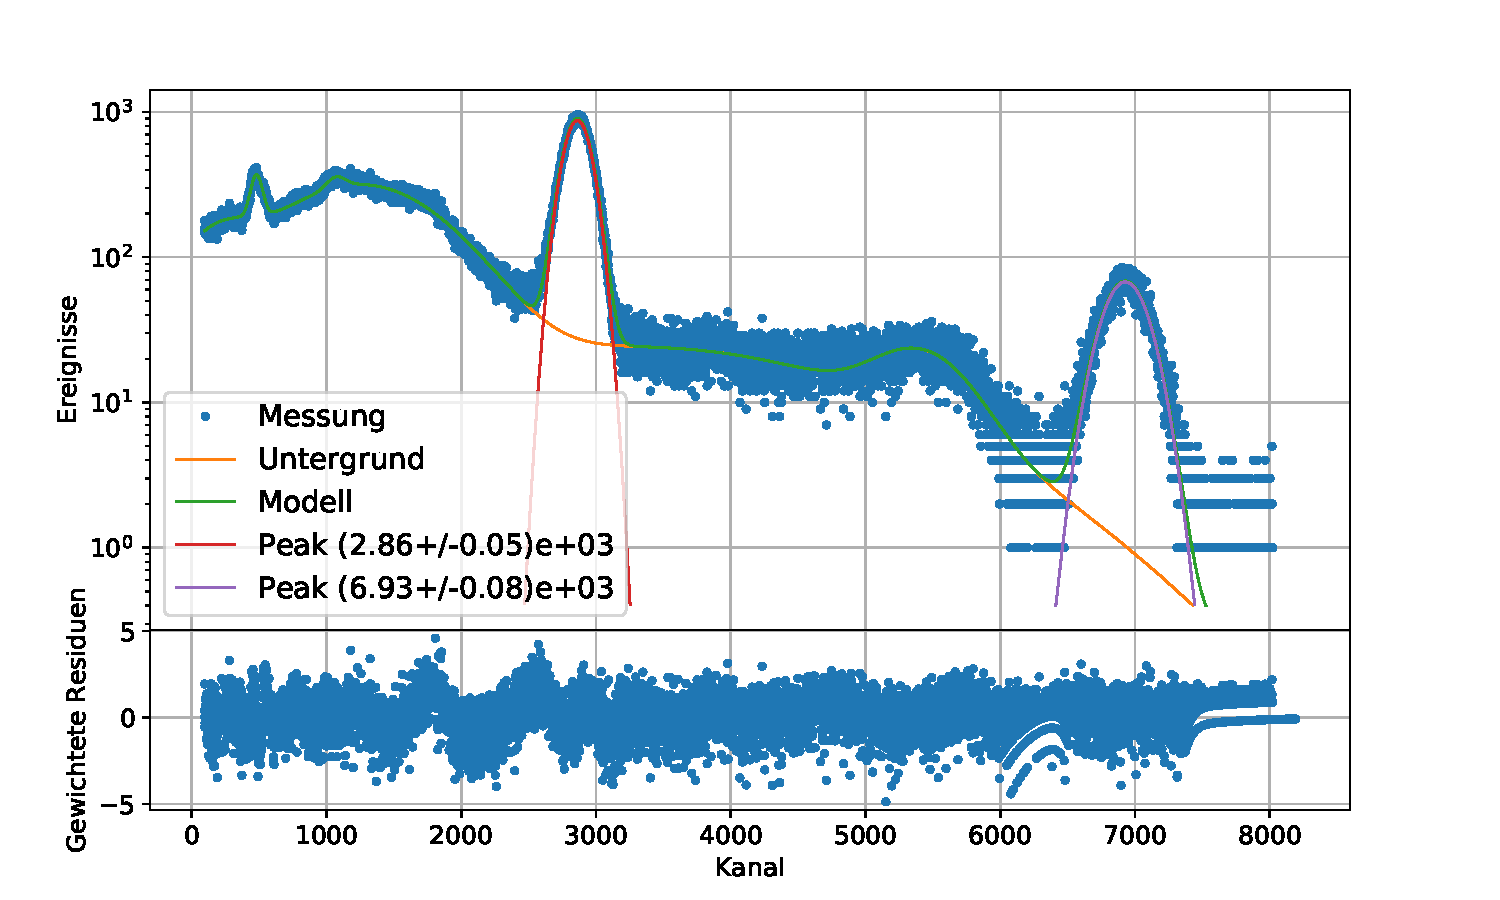
\includegraphics[width= 1 \linewidth]{img/NaNaCh.pdf}
			\subcaption{
				NaI-Detektor.
			}
		\end{subfigure}
		\begin{subfigure}[c]{\textwidth}
			\centering
			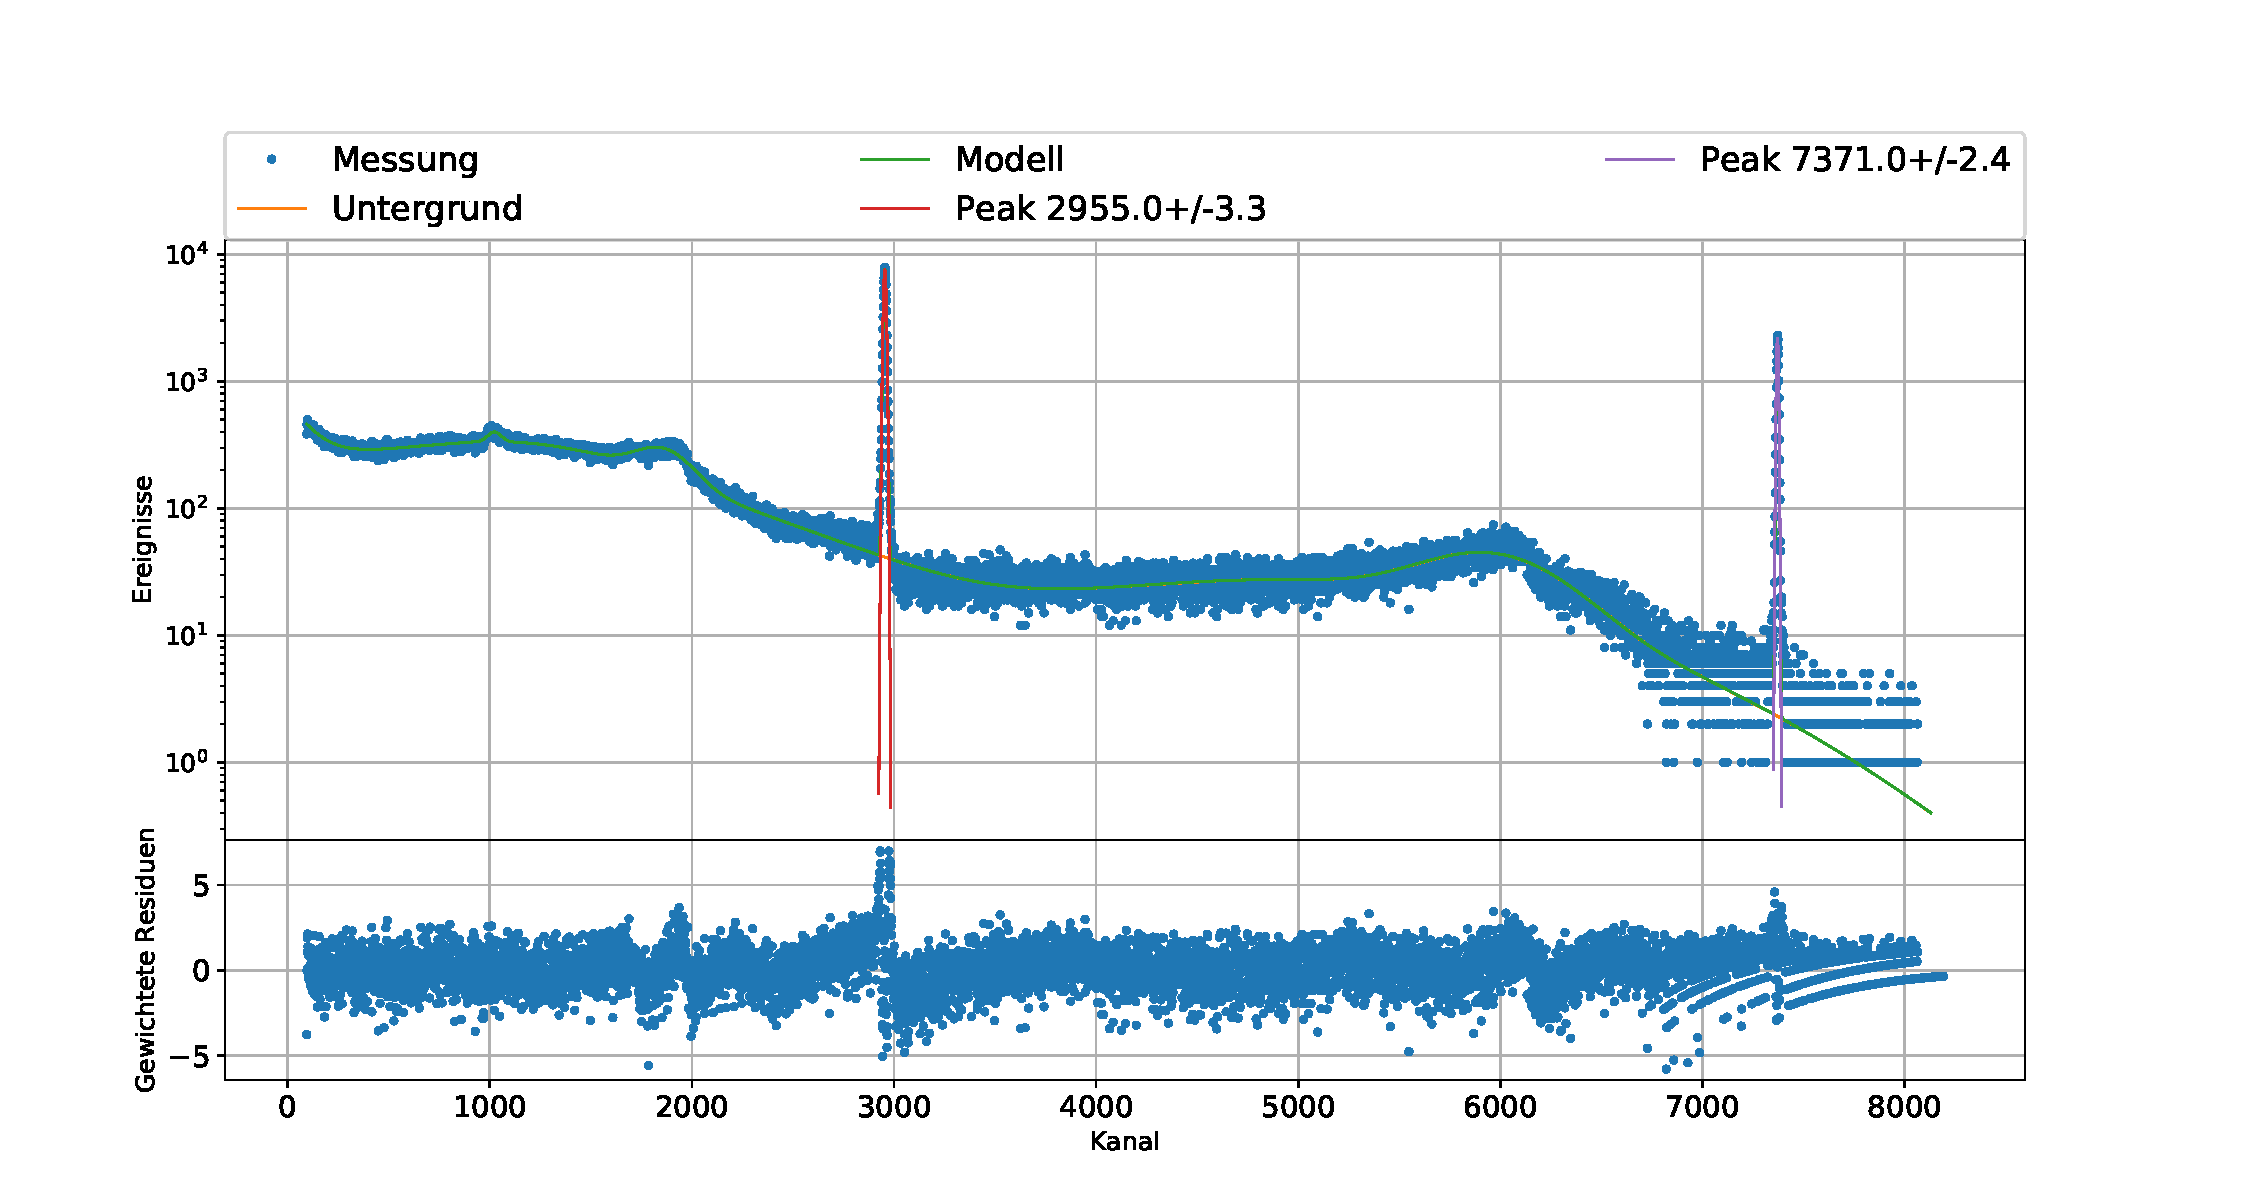
\includegraphics[width= 1 \linewidth]{img/NaGeCh.pdf}
			\subcaption{
				Ge-Detektor.
			}
		\end{subfigure}
		\caption{$^{22}$Na-Probe}
		\label{fg_Na_ch}
	\end{figure}


	\subsubsection{Kalibration}
  Mittels der Literaturwerte der Peaks der $^{22}$Na-Probe (\SI{511}{keV} und \SI{1274}{keV} \cite{Anleitung}) lassen sich die Kanäle umrechnen zu einer Energieskala.  %TODO erläutert in Theorie?
	In \cref{fg_kali_mix} sind in blau(gelb) die zwei Kalibrationspunkte für den NaJ-Detektor(Ge-Detektor) abgebildet.
	Die Unsicherheit des Kanals ist durch die Standardunsicherheit der Gaußkurve in \cref{fg_Na_ch} gegeben.

	\begin{figure}[H]
			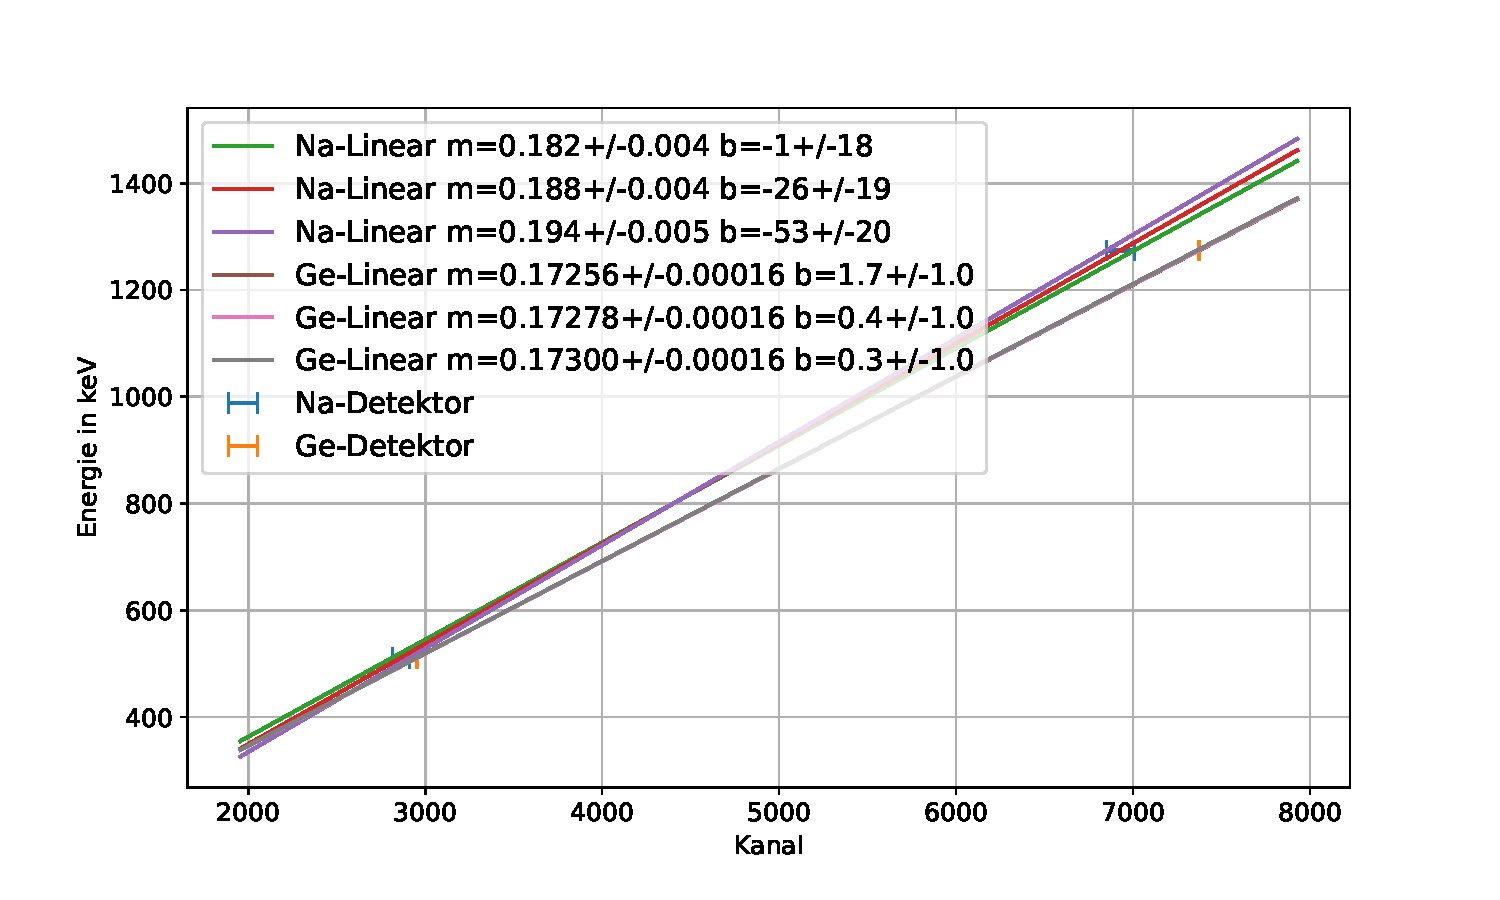
\includegraphics[width= 0.8 \linewidth]{img/kali_mix.pdf}
			\caption{
				Kalibrationsgeraden $f(x)=mx+b$.
				$m$ ist die Steigung der Gerade in \si{keV}.
				$b$ ist der y-Achsenabschnitt in \si{keV}.
			}
			\label{fg_kali_mix}
	\end{figure}

	Da ein linearer Fit zwischen zwei Punkten mit Unsicherheiten mit dem \enquote{Least-Square-Fit} nicht zielführend ist, werden drei Geraden durch die Messintervalle gelegt, sodass sich eine mittlere, maximale und minimale Steigung ergeben.
	Eine Mittelung dieser Werte ist in \cref{tb_kali_avg} aufgeführt.

\begin{table}[H]
		\centering
		\begin{tabular}{c | c | c  }
			 Detektor& $m$ in \si{kev}& $b$ in \si{keV} \\ \hline
			 NaI & \SI{0.188+-0.015}{} & \SI{-30+-60}{} \\
			 Ge & \SI{0.1728+-0.0006}{} & \SI{1.3+-2.3}{} \\
		\end{tabular}
		\caption{
		Gemittelte Kalibrationsparameter für NaJ- und Ge-Detektor.
		}
		\label{tb_kali_avg}
\end{table}
%TODO y-Achse ist ca. Null, nice, aber diskutieren warum Anfang alles Null?
Damit lässt sich ein Kanal $c$ nach \cref{eq_trans} in die Energie $E$ transformieren.
\begin{equation}
	\label{eq_trans}
	E = m\cdot c + b
\end{equation}

\subsection{Peaks und Kanten}
In \crefrange{fg_Na}{fg_Mix} sind die kalibrierten Spektren von vier Proben für jeden der Detektoren dargestellt.
Die horizontalen Linien die sich im höher energetischen Bereich ergeben entstehen durch die logarithmischen Darstellung.

%TODO In der Theorie?
Die Comptonkante berechnet sich aus dem Literaturwert:
\begin{equation}
	E_c = E_\gamma - \frac{E_\gamma }{1+2E_\gamma/m_ec^2}
\end{equation}
Die Rückstreukante ist analog:
\begin{equation}
	E_c =  \frac{E_\gamma}{1+E_\gamma/m_ec^2}
\end{equation}
Die Literaturwert stammen aus \cite{Anleitung}.
Außerdem wurden die Ränder des Bereichs der Röntgenfluoreszenz von Blei gekennzeichnet (aus \cite{XRAYDB}).


%TODO caption ? Unsicherheit?
\begin{figure}[H]
		\centering
		\begin{subfigure}[c]{\textwidth}
			\centering
			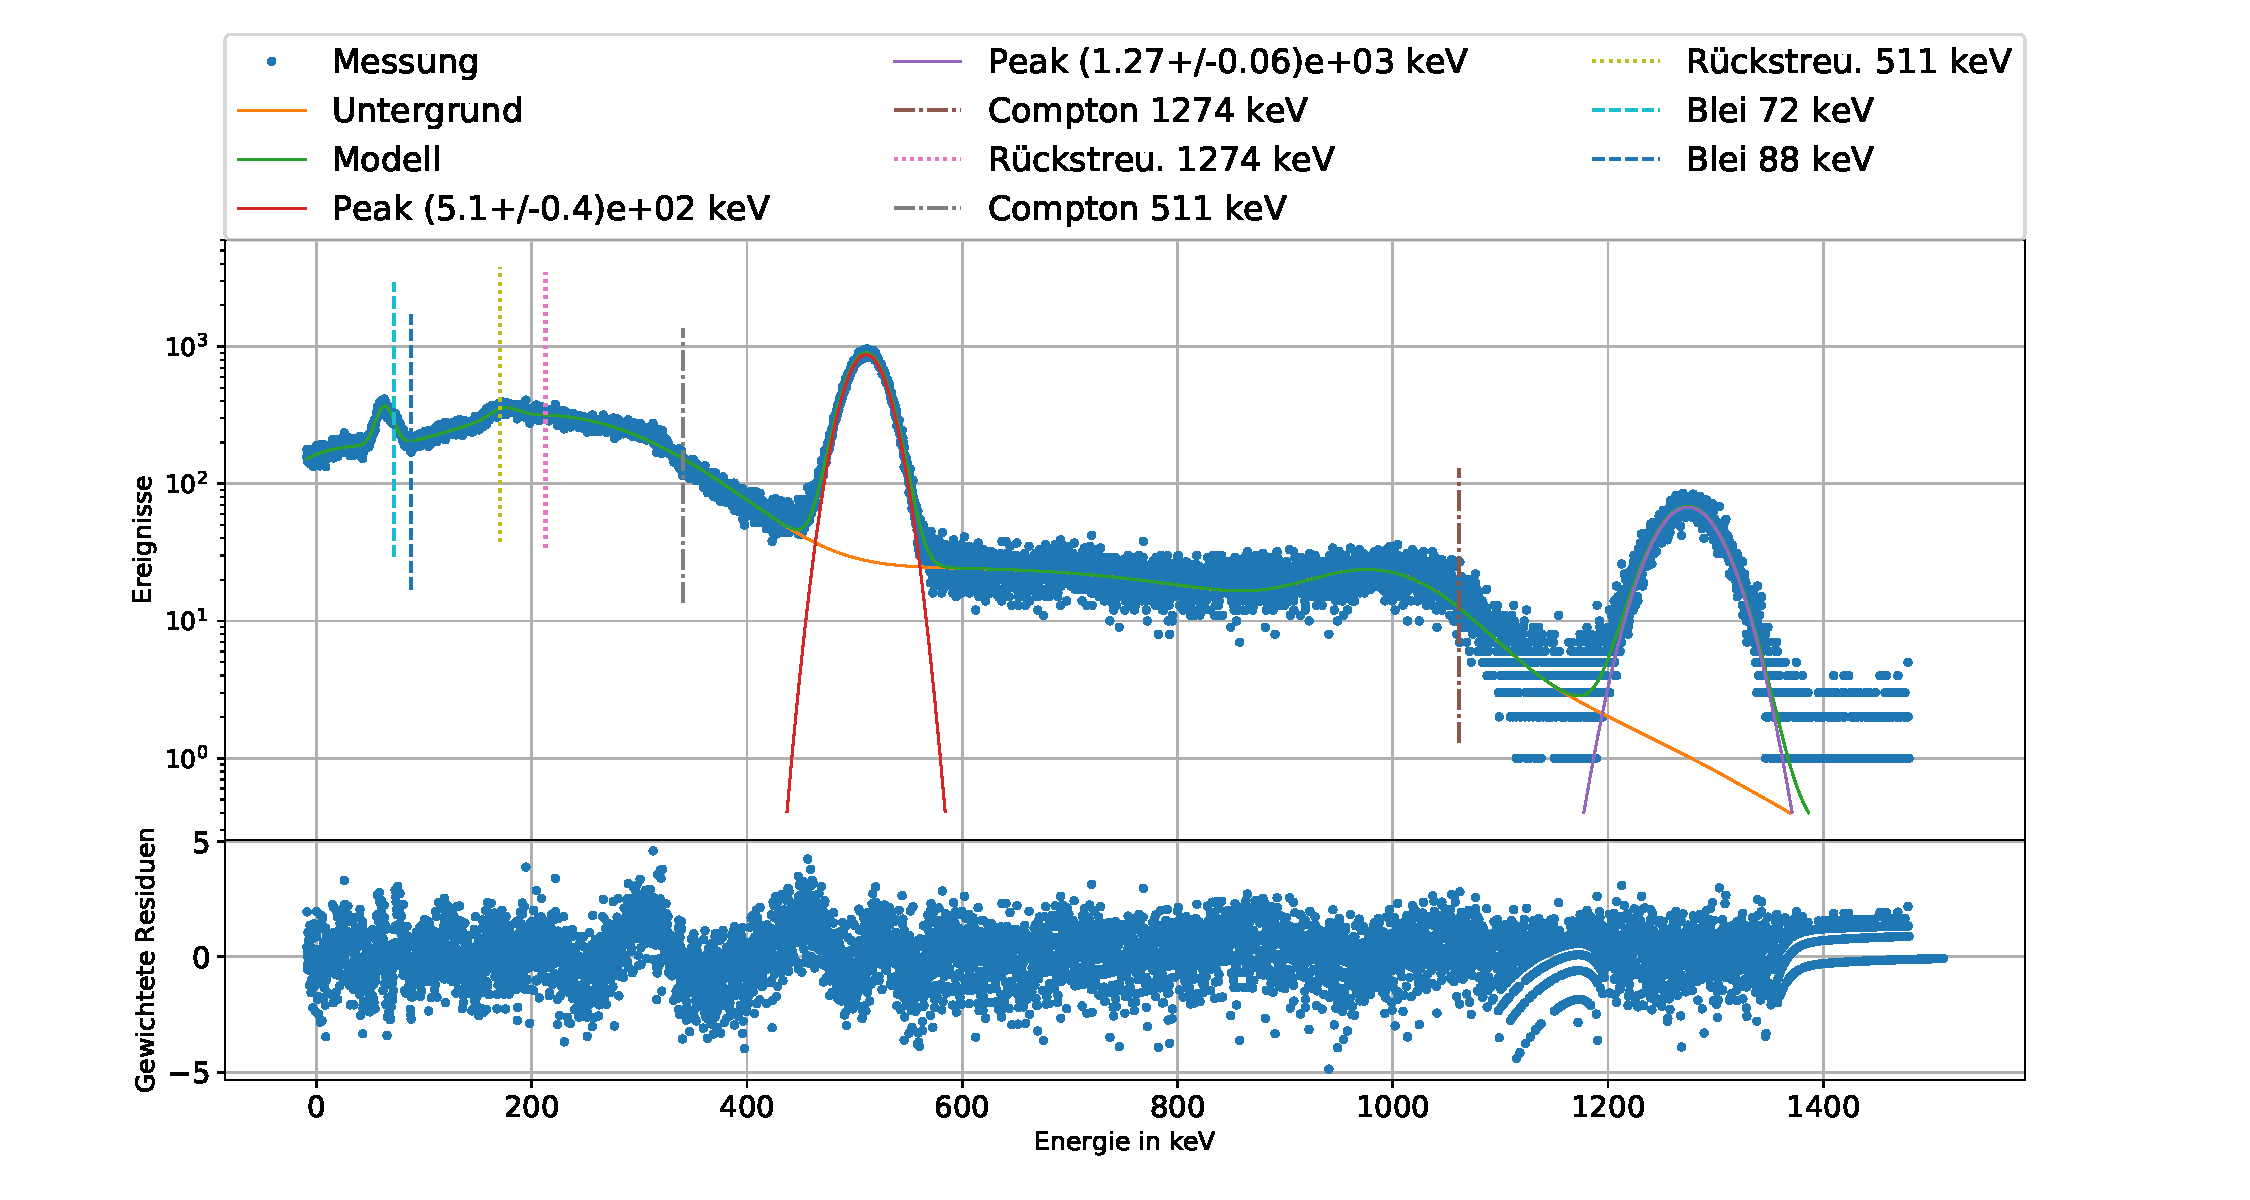
\includegraphics[width= 1 \linewidth]{img/NaNa.pdf}
			\subcaption{
				NaI-Detektor.
			}
		\end{subfigure}
		\begin{subfigure}[c]{\textwidth}
			\centering
			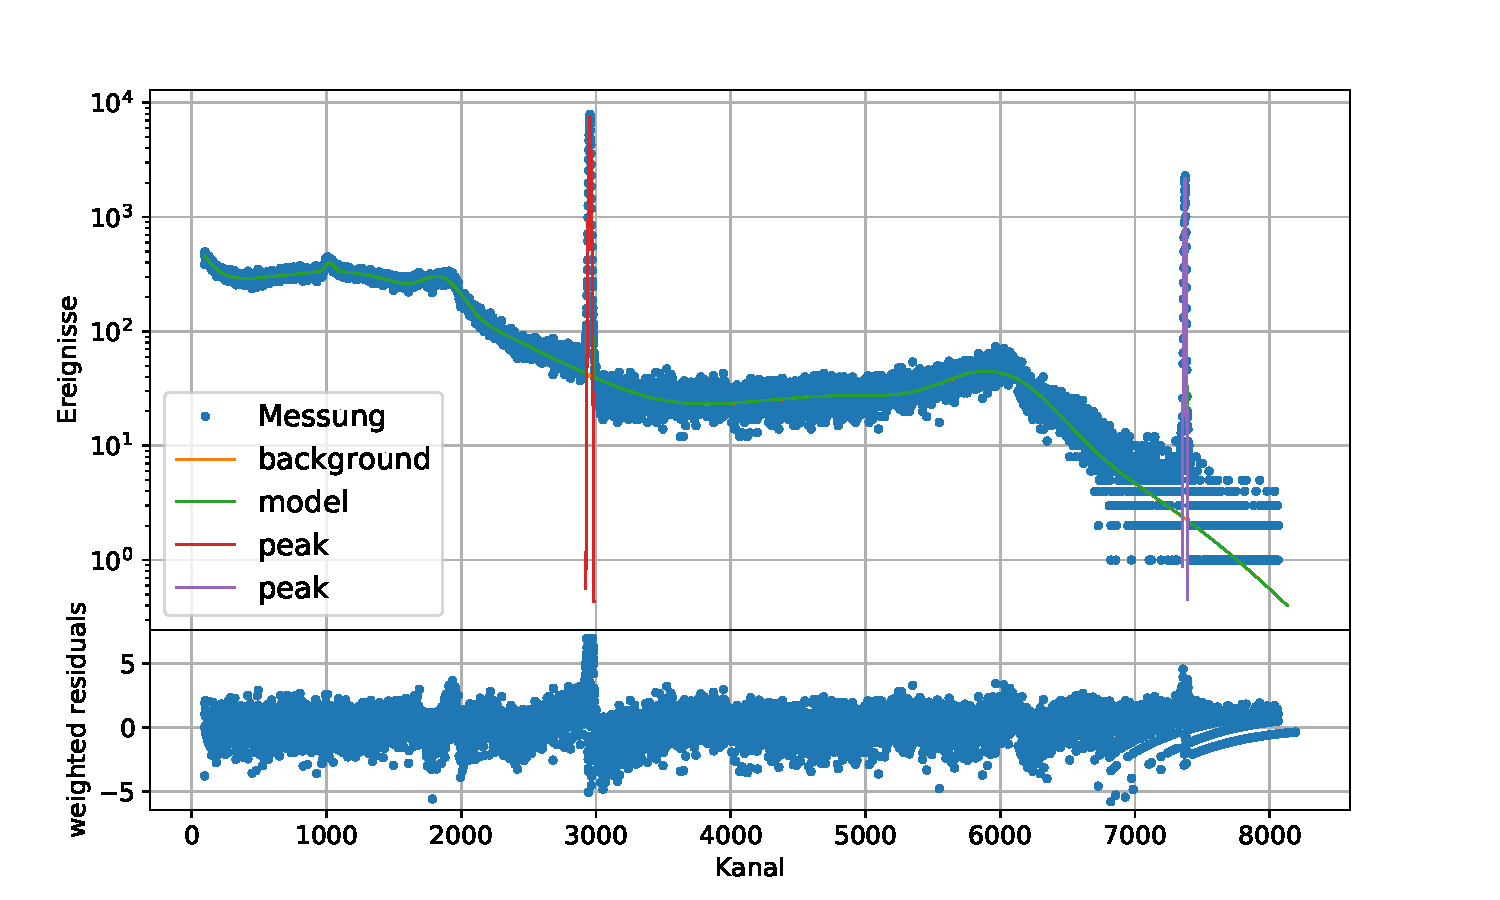
\includegraphics[width= 1 \linewidth]{img/NaGe.pdf}
			\subcaption{
				Ge-Detektor.
			}
		\end{subfigure}
		\caption{$^{22}$Na-Probe}
		\label{fg_Na}
	\end{figure}


\begin{figure}[H]
		\centering
		\begin{subfigure}[c]{\textwidth}
			\centering
			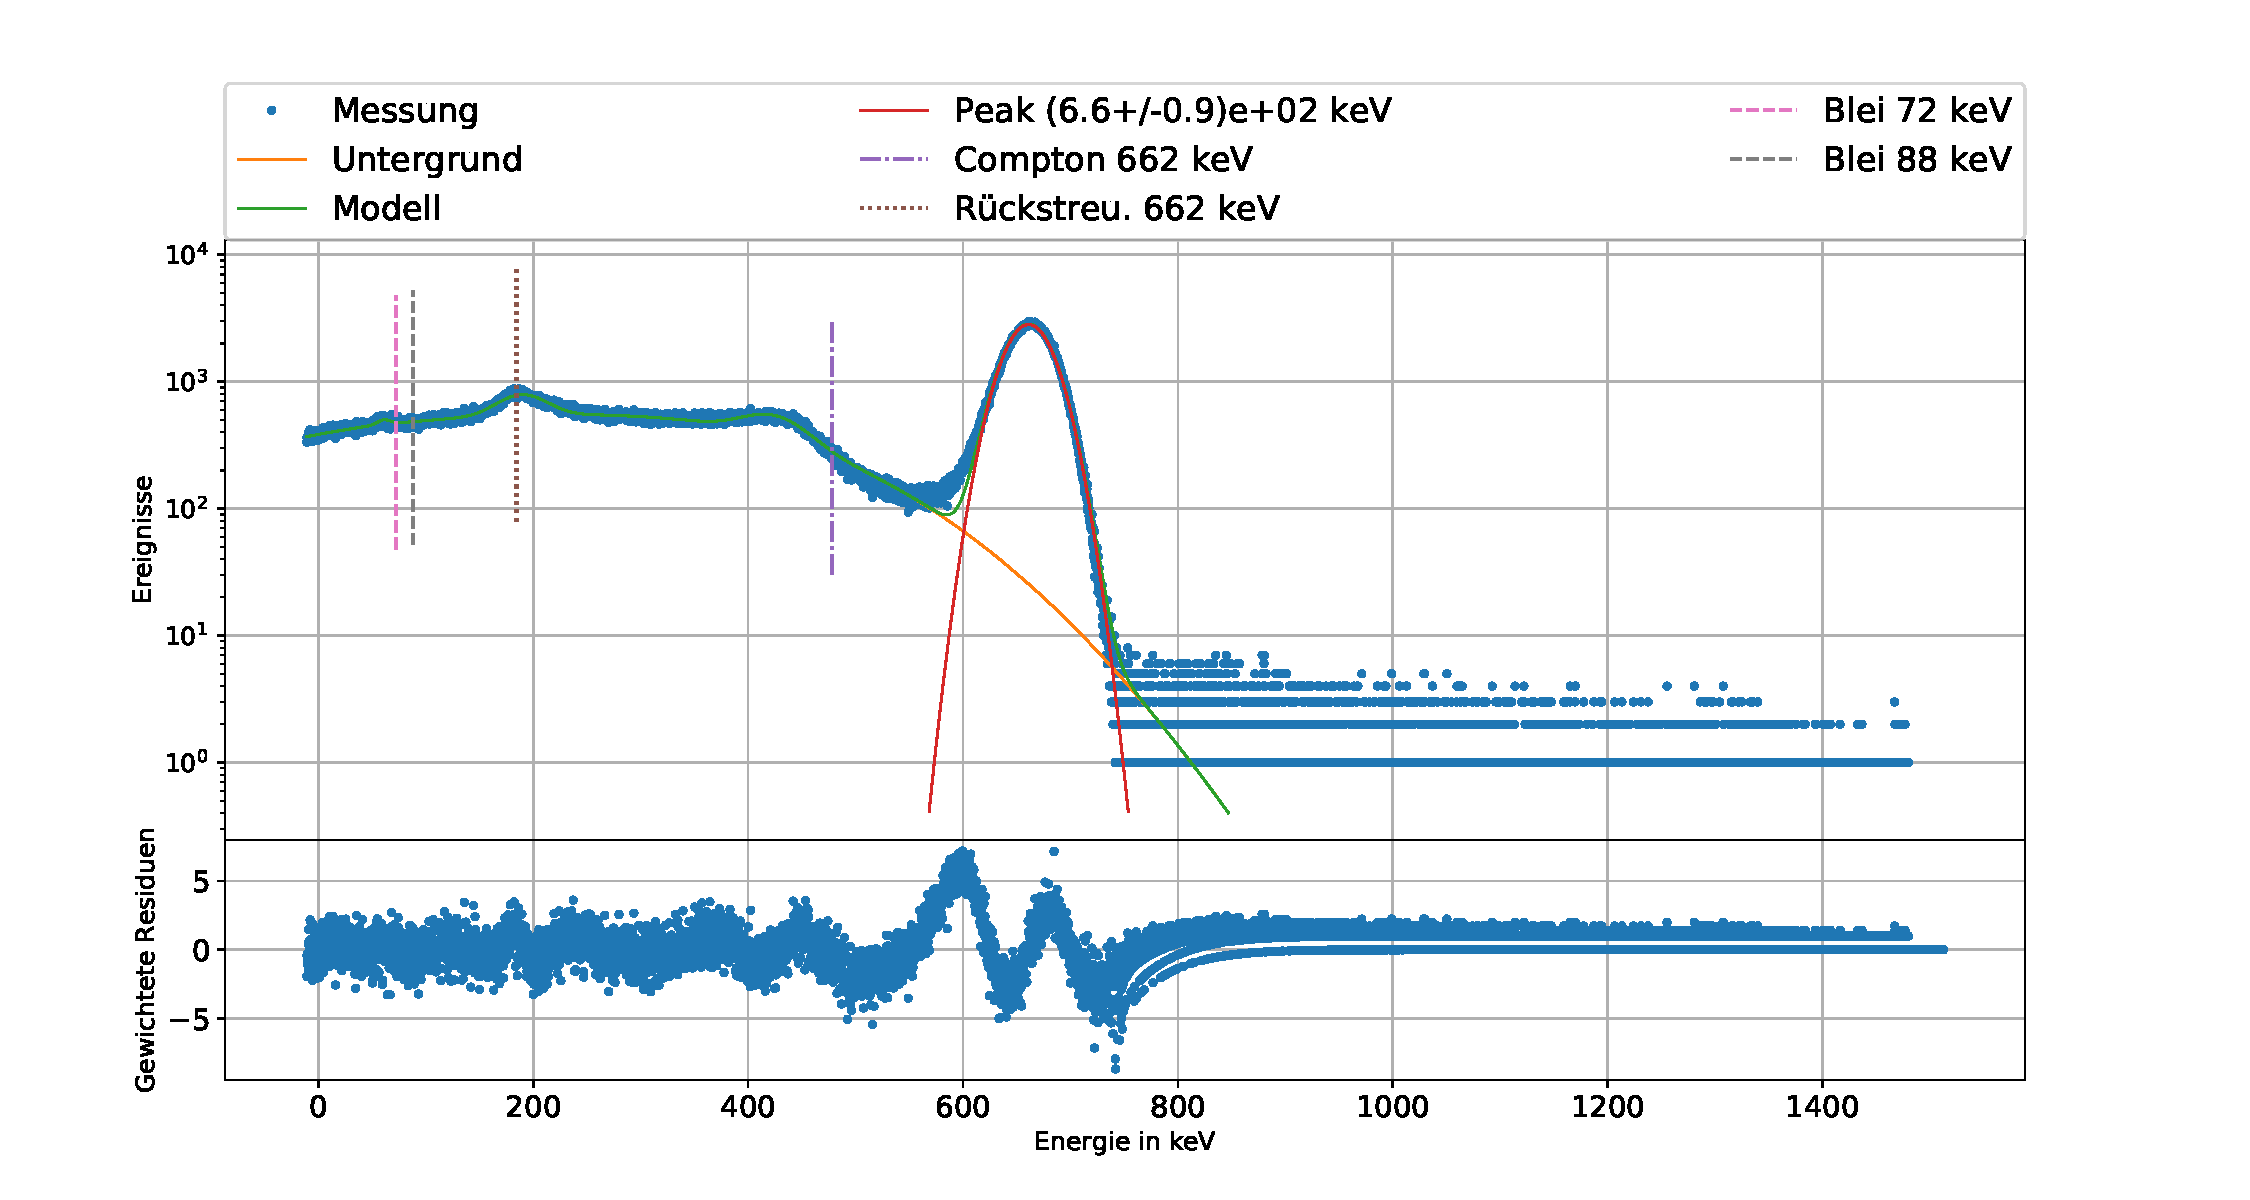
\includegraphics[width= 1 \linewidth]{img/CsNa.pdf}
			\subcaption{
				NaI-Detektor.
			}
		\end{subfigure}
		\begin{subfigure}[c]{\textwidth}
			\centering
			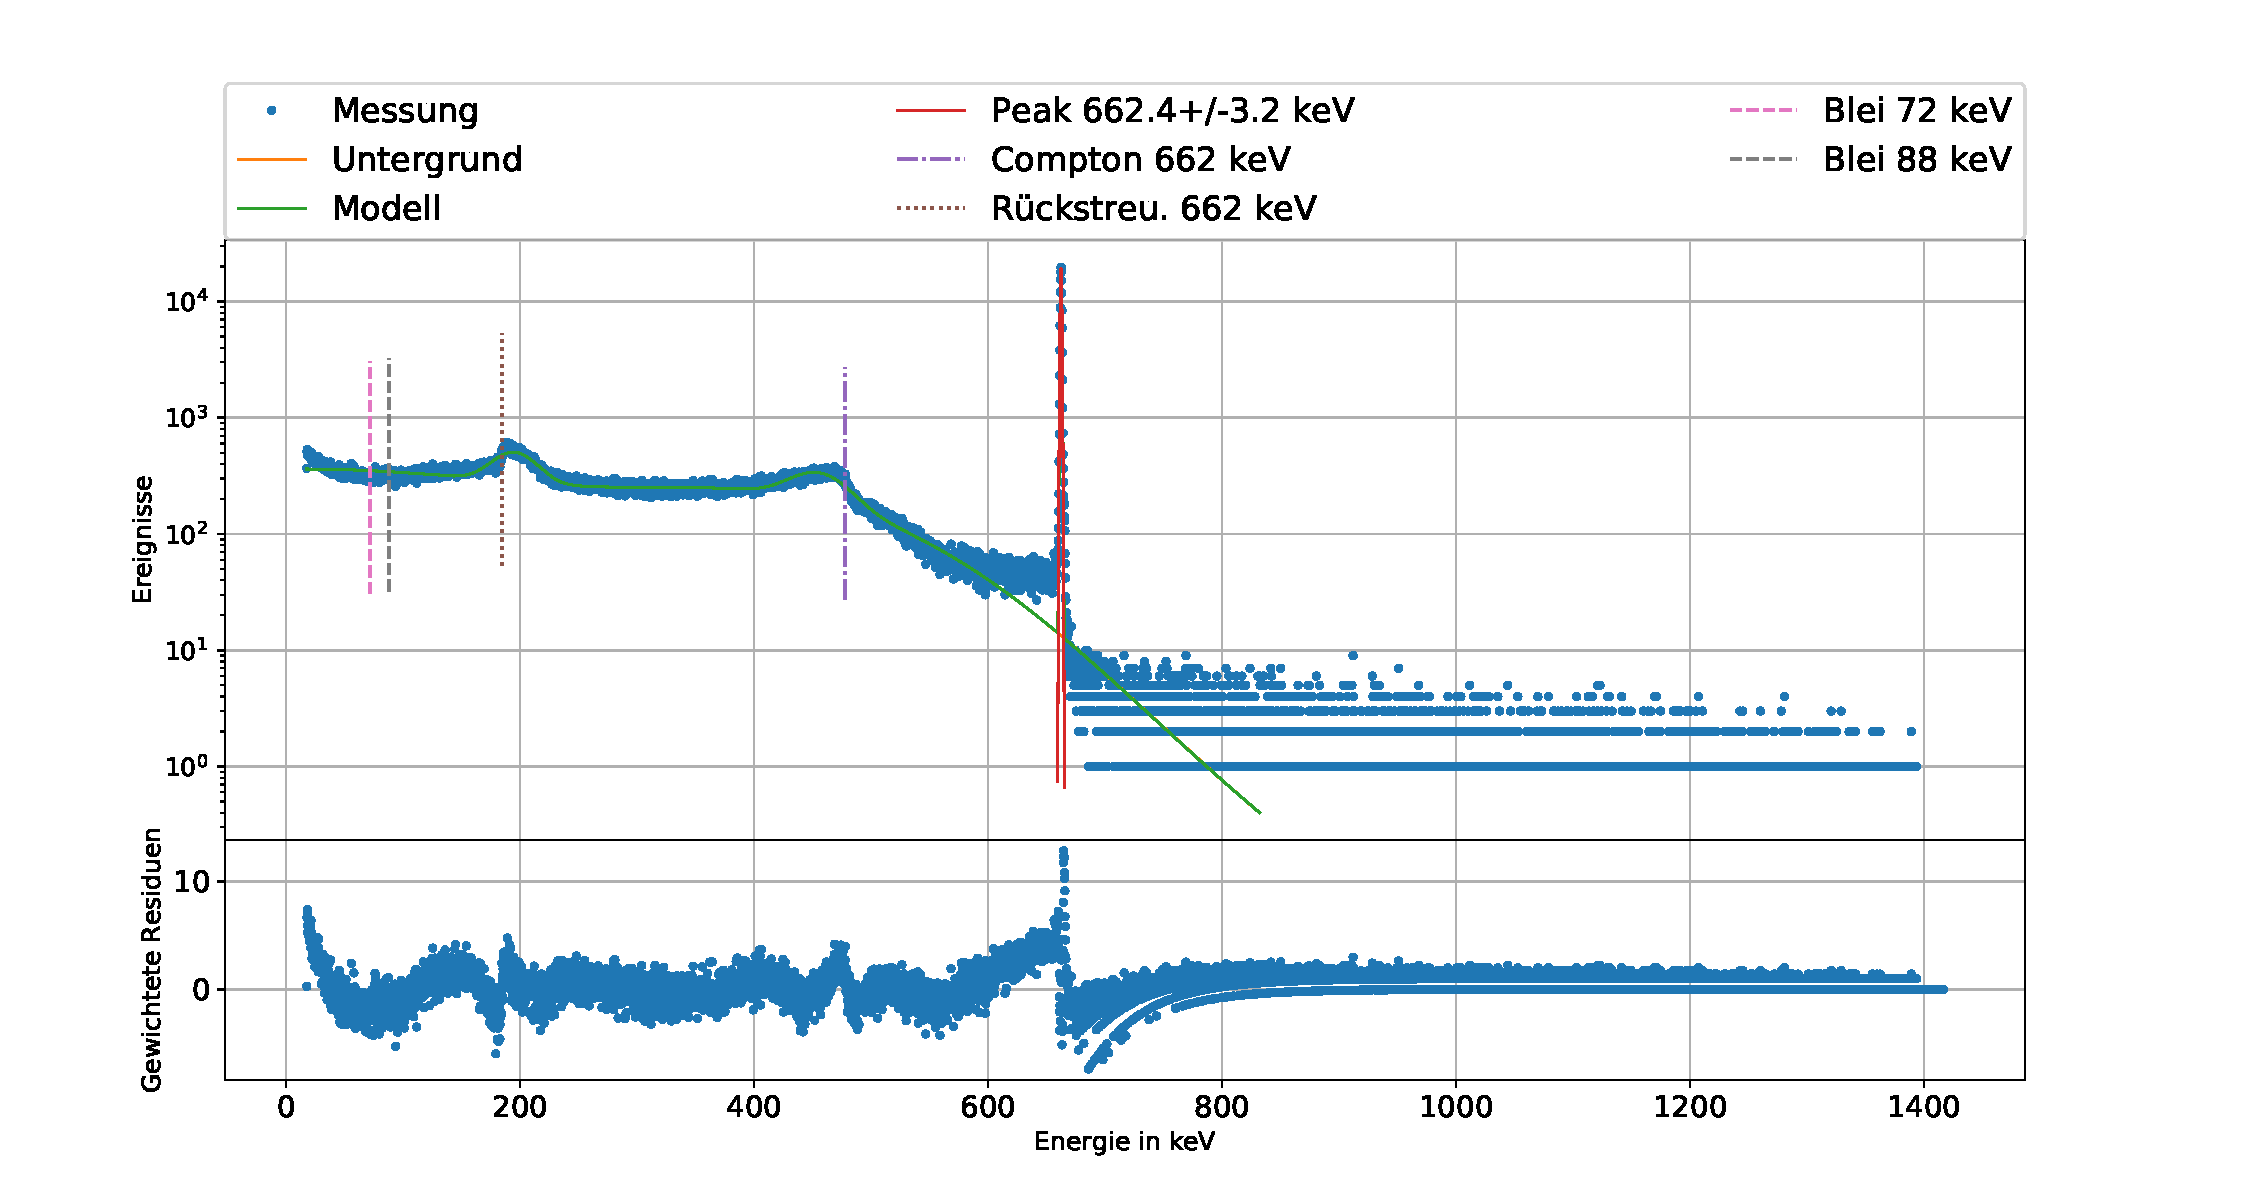
\includegraphics[width= 1 \linewidth]{img/CsGe.pdf}
			\subcaption{
				Ge-Detektor.
			}
		\end{subfigure}
		\caption{$^{137}$Cs-Probe}
		\label{fg_Cs}
	\end{figure}

\begin{figure}[H]
		\centering
		\begin{subfigure}[c]{\textwidth}
			\centering
			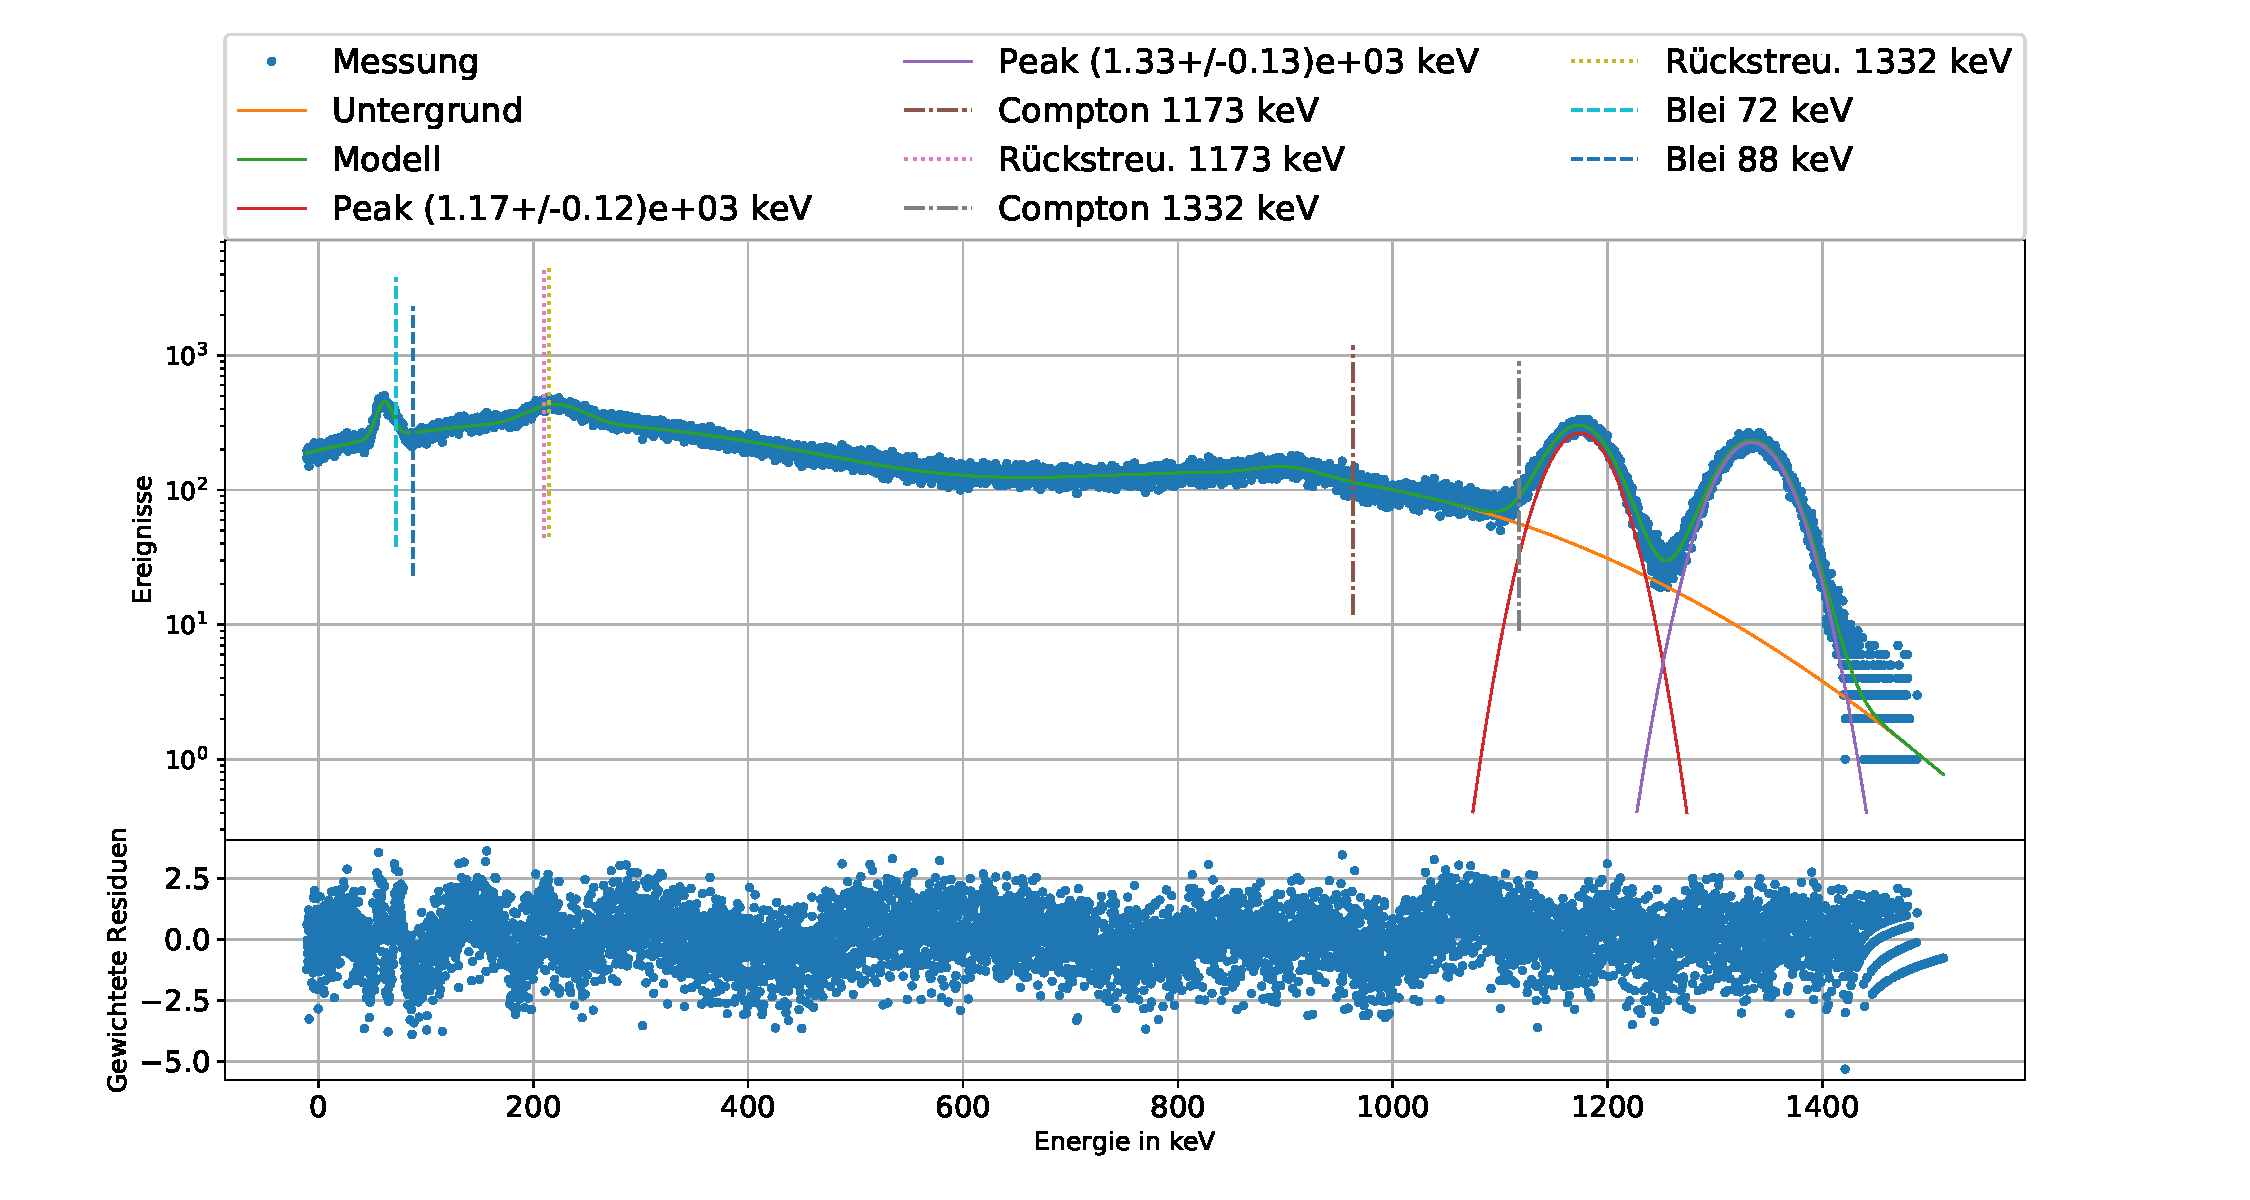
\includegraphics[width= 1 \linewidth]{img/CoNa.pdf}
			\subcaption{
				NaI-Detektor.
			}
		\end{subfigure}
		\begin{subfigure}[c]{\textwidth}
			\centering
			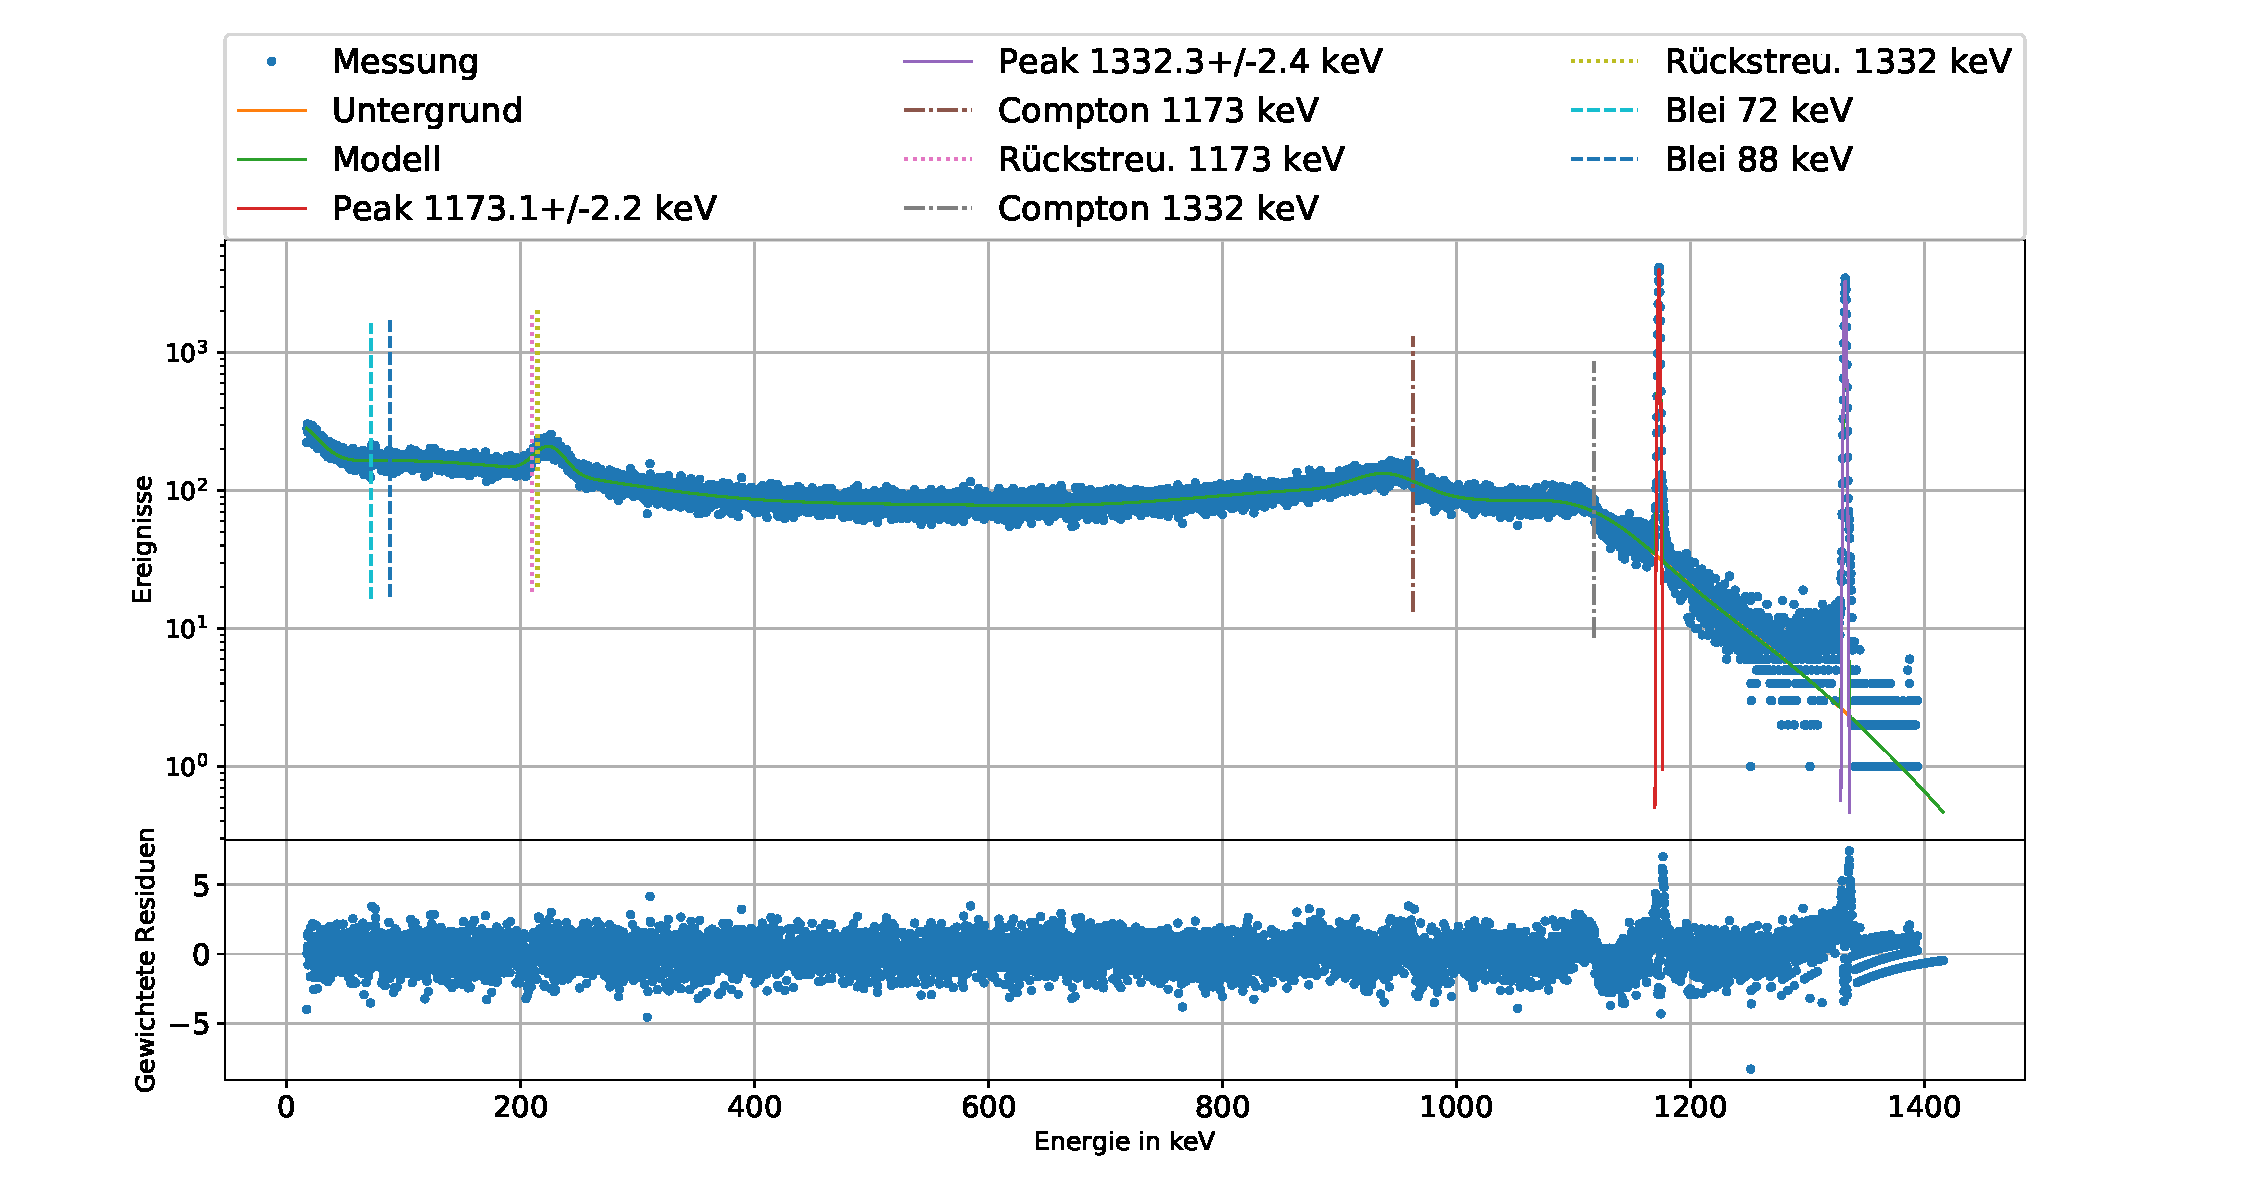
\includegraphics[width= 1 \linewidth]{img/CoGe.pdf}
			\subcaption{
				Ge-Detektor.
			}
		\end{subfigure}
		\caption{$^{57}$Co-Probe}
		\label{fg_Na}
	\end{figure}

\begin{figure}[H]
		\centering
		\begin{subfigure}[c]{\textwidth}
			\centering
			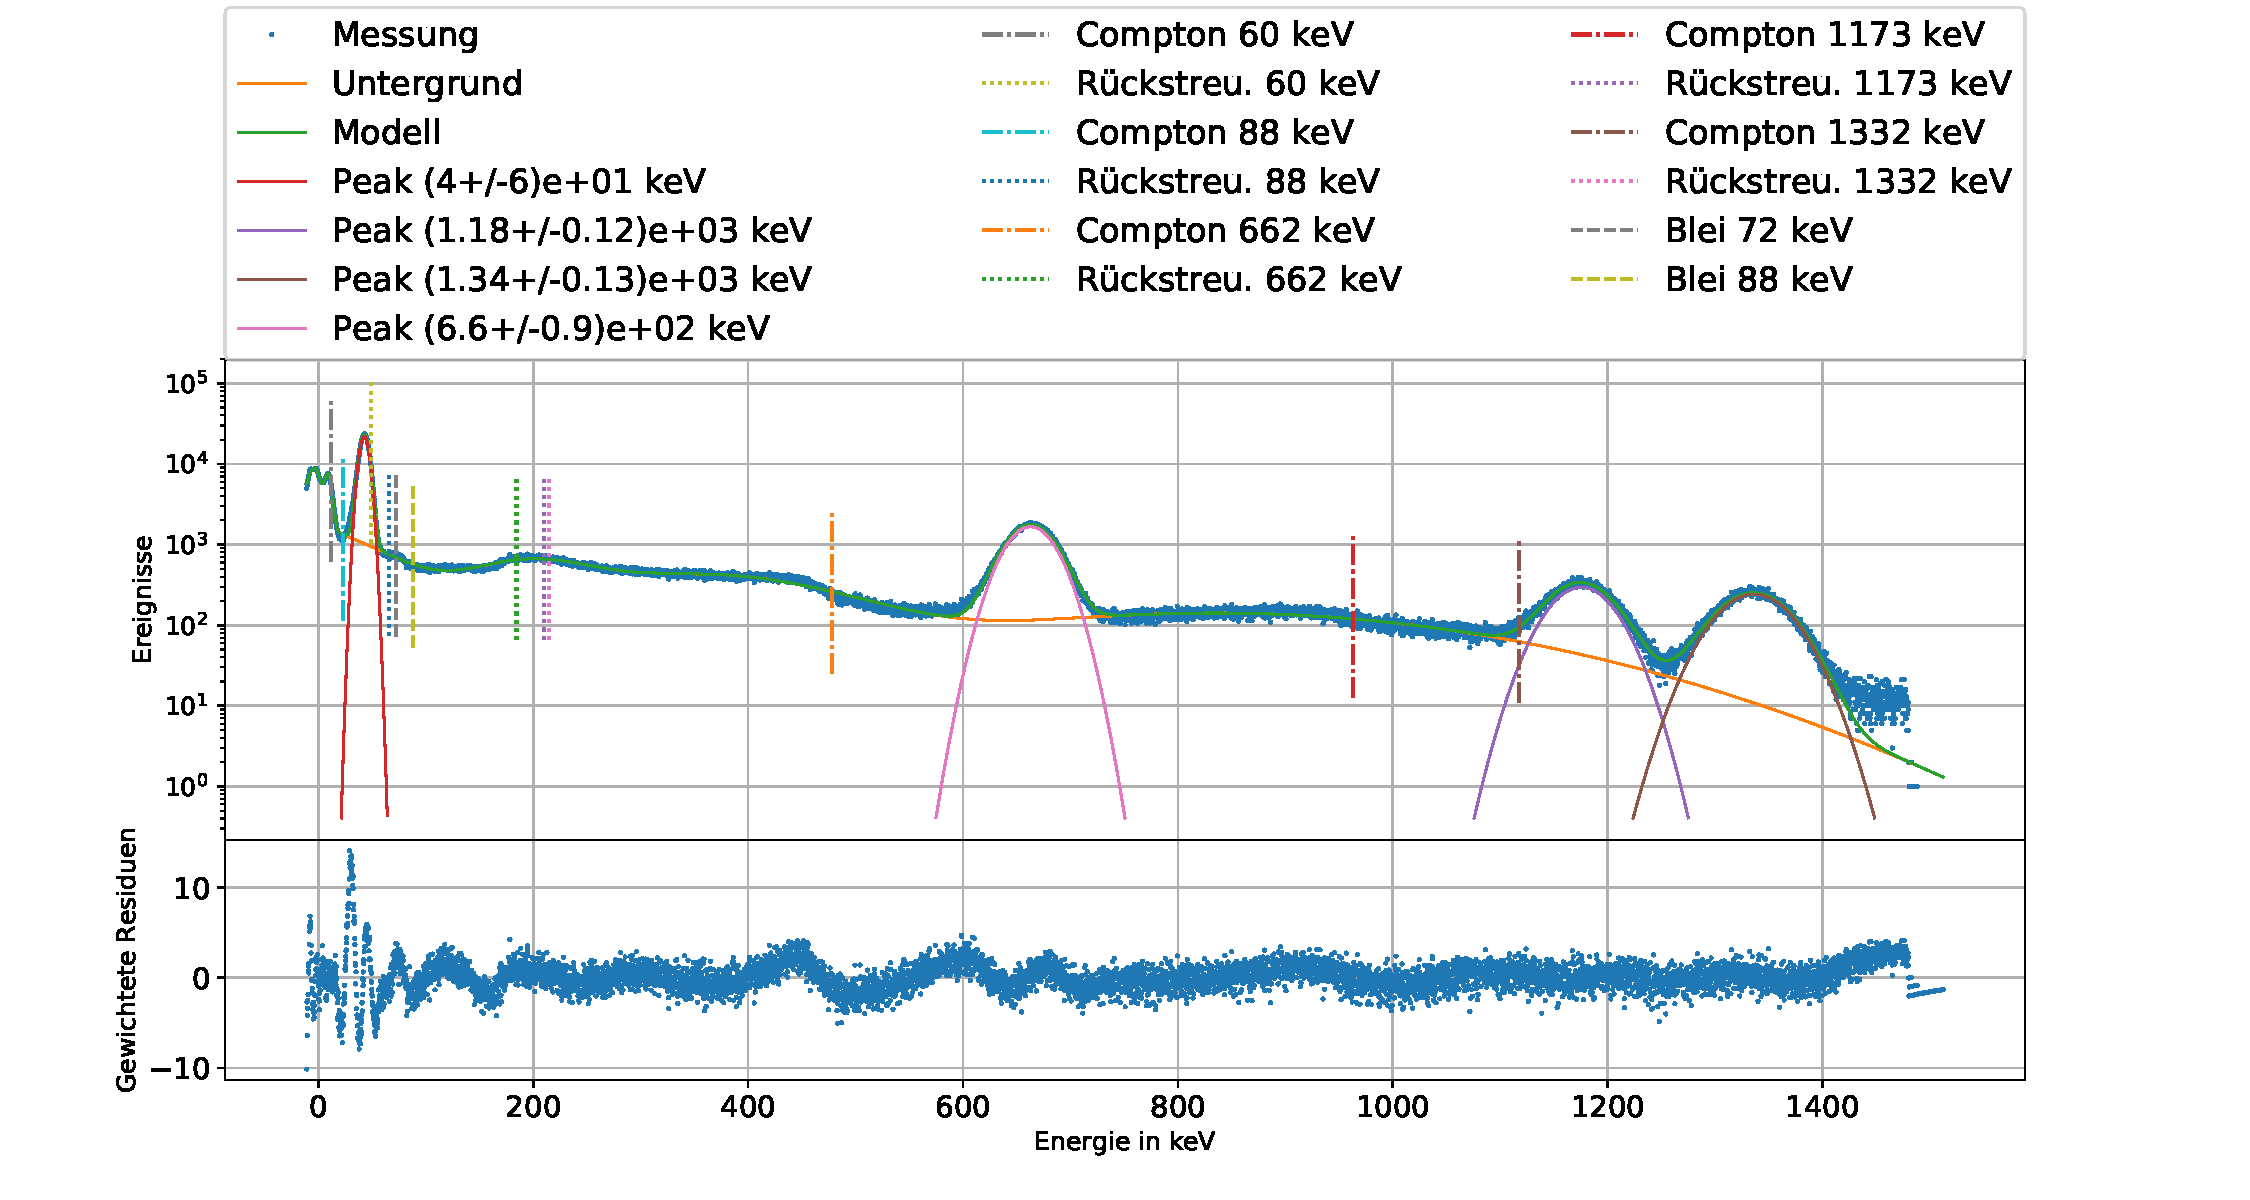
\includegraphics[width= 1 \linewidth]{img/MixNa.pdf}
			\subcaption{
				NaI-Detektor.
			}
		\end{subfigure}
		\begin{subfigure}[c]{\textwidth}
			\centering
			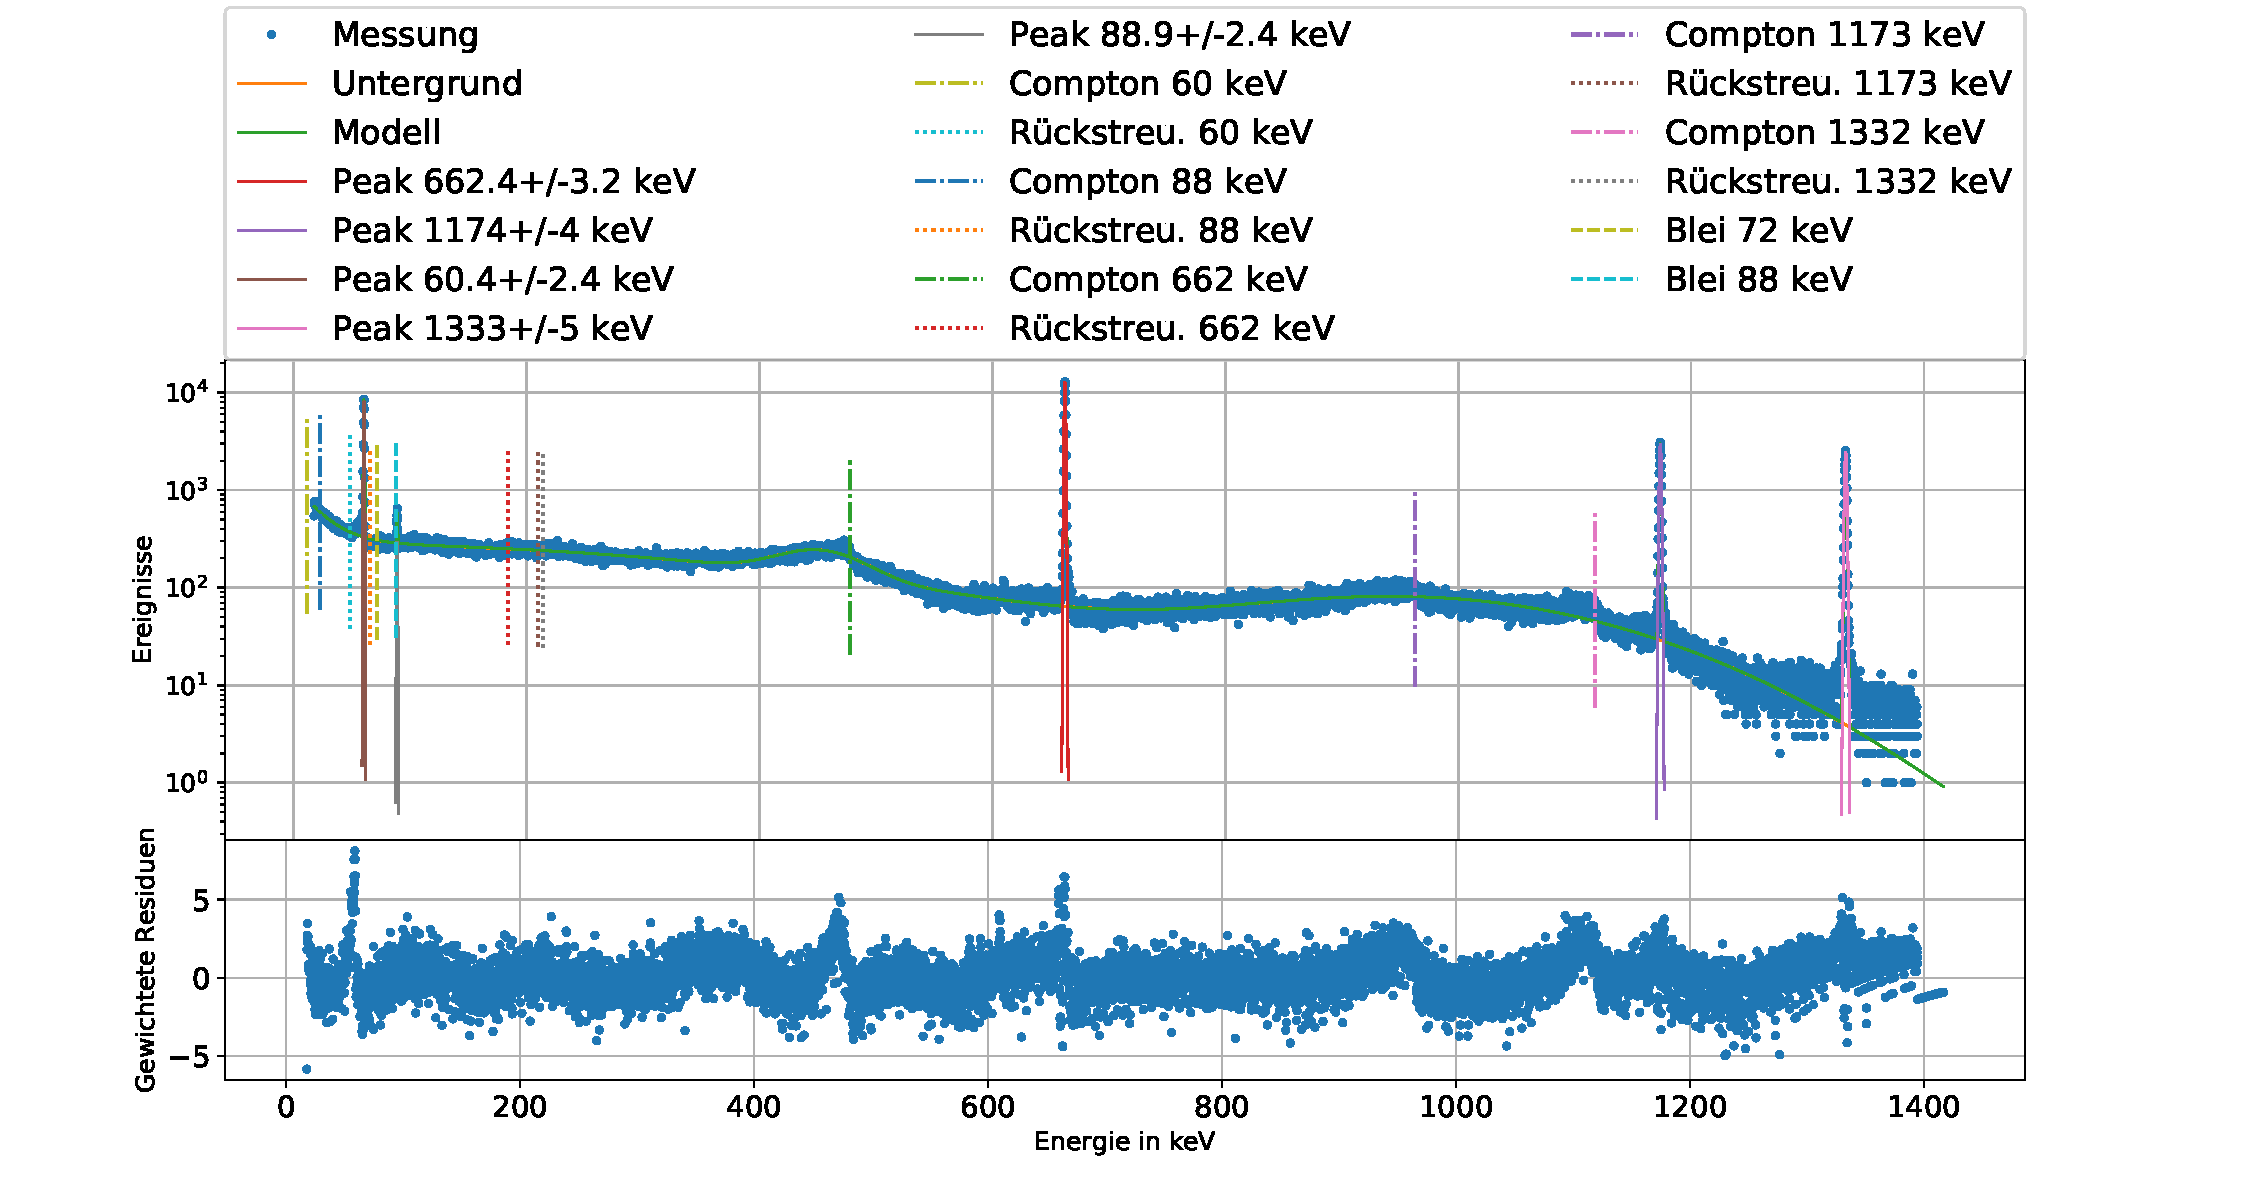
\includegraphics[width= 1 \linewidth]{img/MixGe.pdf}
			\subcaption{
				Ge-Detektor.
			}
		\end{subfigure}
		\caption{Misch-Probe}
		\label{fg_Mix}
	\end{figure}


\subsection{Erzprobe}
\subsection{Nichtlinearität des Detektors}
Die Nichtlinearität des Detektors kann gezeigt werden, in dem man die relative Differenz der gemessenen Peaks gegen den Referenzwert des Peaks aufträgt.
Also
\begin{equation}
	\delta(E_r) = 1- \frac{E_m}{E_r}
\end{equation}
Diese wurde  in \cref{fg_diff_na} und \cref{fg_diff_ge} für NaI- und Ge-Detektor dargestellt.
$E_r$ ist Literaturwert für die Peakposition und $E_m$ ist der gemessenen Wert.

%TODO log plot hier von?
\begin{figure}[H]
		\centering
		\begin{subfigure}[t]{0.8\textwidth}
			\centering
			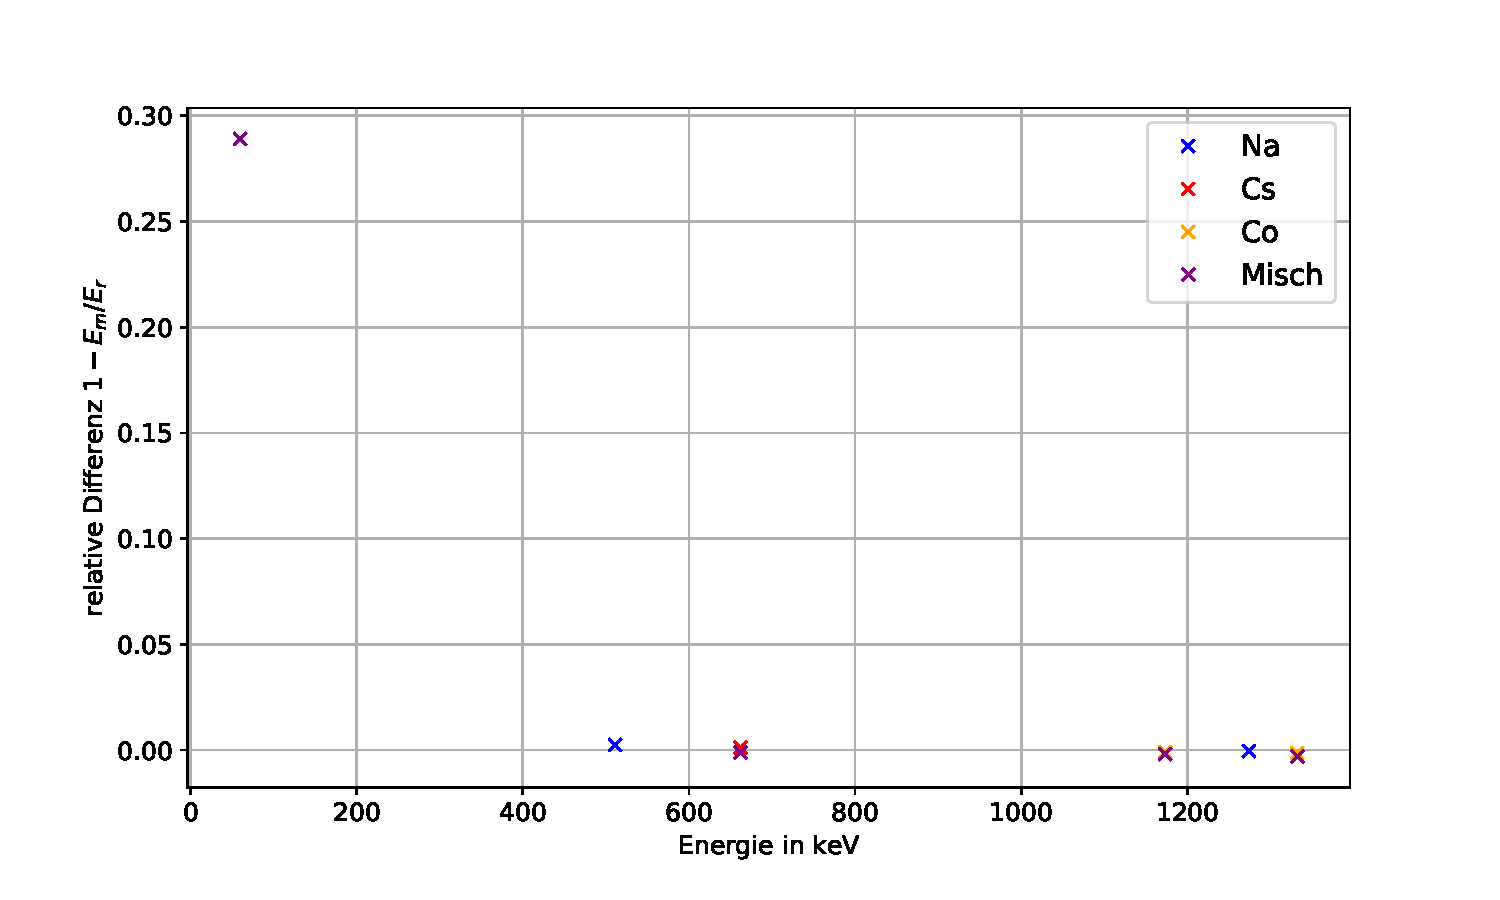
\includegraphics[width= \linewidth]{img/diff_na.pdf}
			\subcaption{
				relative Differenz.
			}
		\end{subfigure}
		\begin{subfigure}[t]{0.8\textwidth}
			\centering
			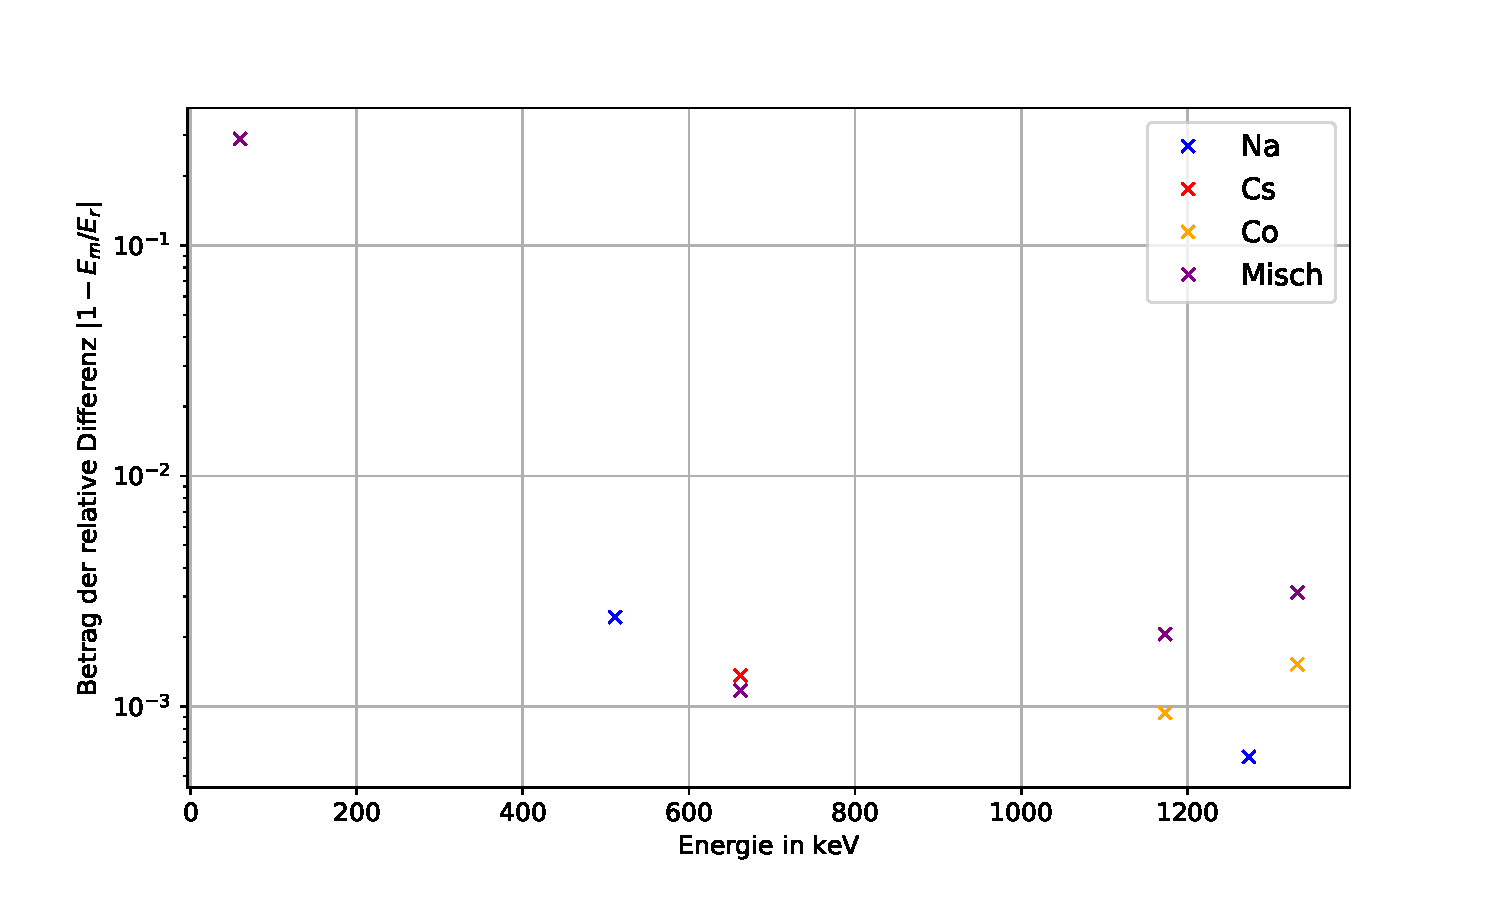
\includegraphics[width=\linewidth]{img/diff_na_log.pdf}
			\subcaption{
				Betrag der relativen Differenz in logarithmischer Darstellung.
			}
		\end{subfigure}
		\caption{Nichtlinearität des NaI-Detektors.
		Die Unsicherheiten sind nicht abgebildet, da ein Abbilden dieser ein Unterscheiden der Werte unmöglich macht.
		Der Wert Null für die relative Differenz liegt immer im Unsicherheitsintervall.
		}
		\label{fg_diff_na}
	\end{figure}
\begin{figure}[H]
		\centering
		\begin{subfigure}[t]{0.8\textwidth}
			\centering
			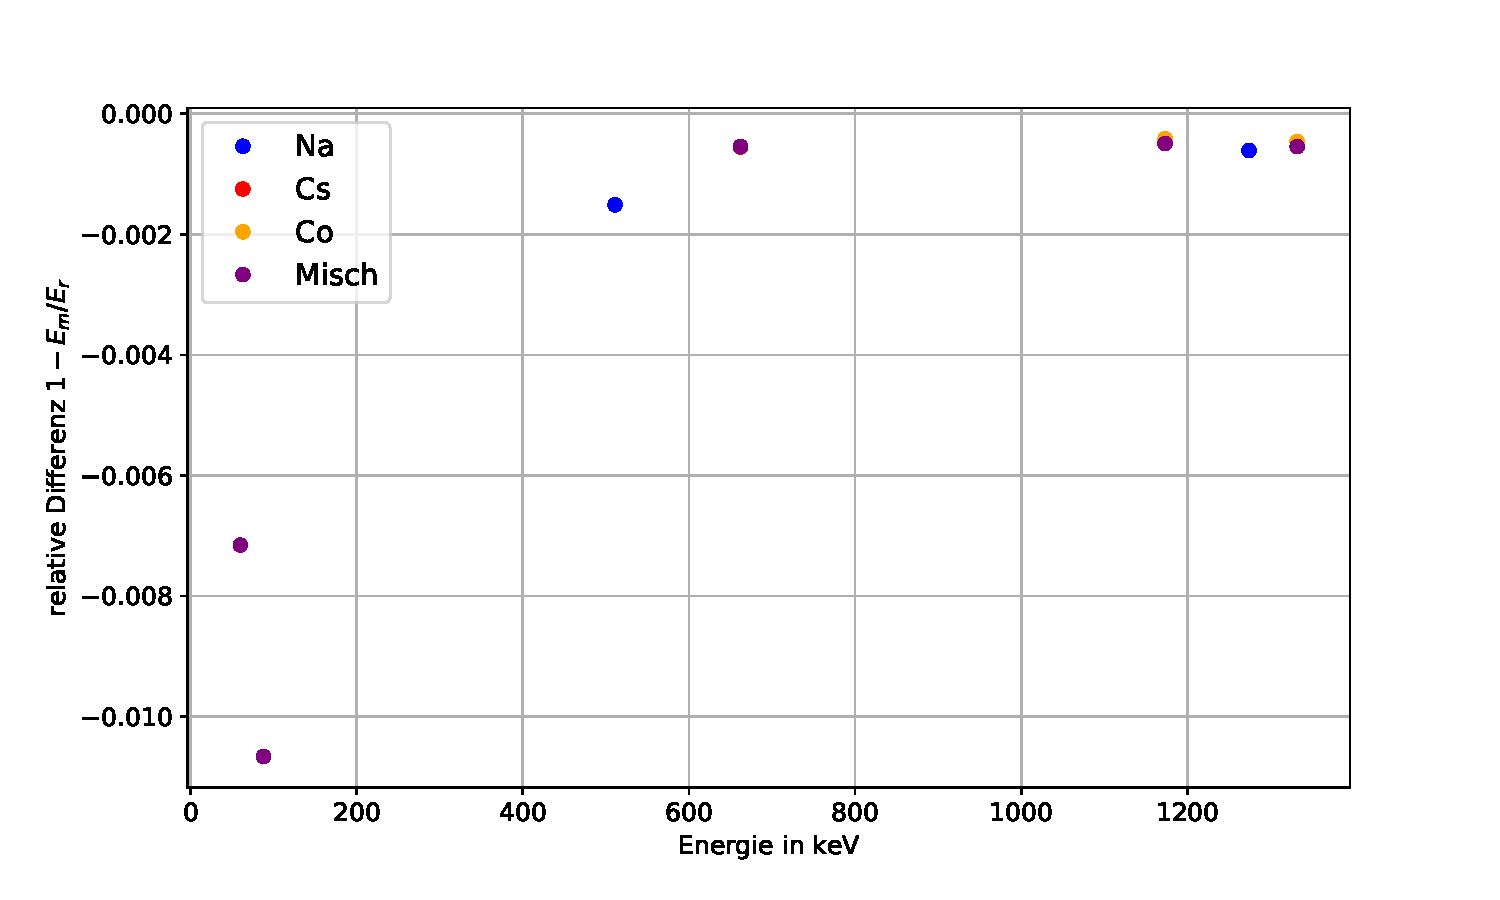
\includegraphics[width= \linewidth]{img/diff_ge.pdf}
			\subcaption{
				relative Differenz.
			}
		\end{subfigure}
		\begin{subfigure}[t]{0.8\textwidth}
			\centering
			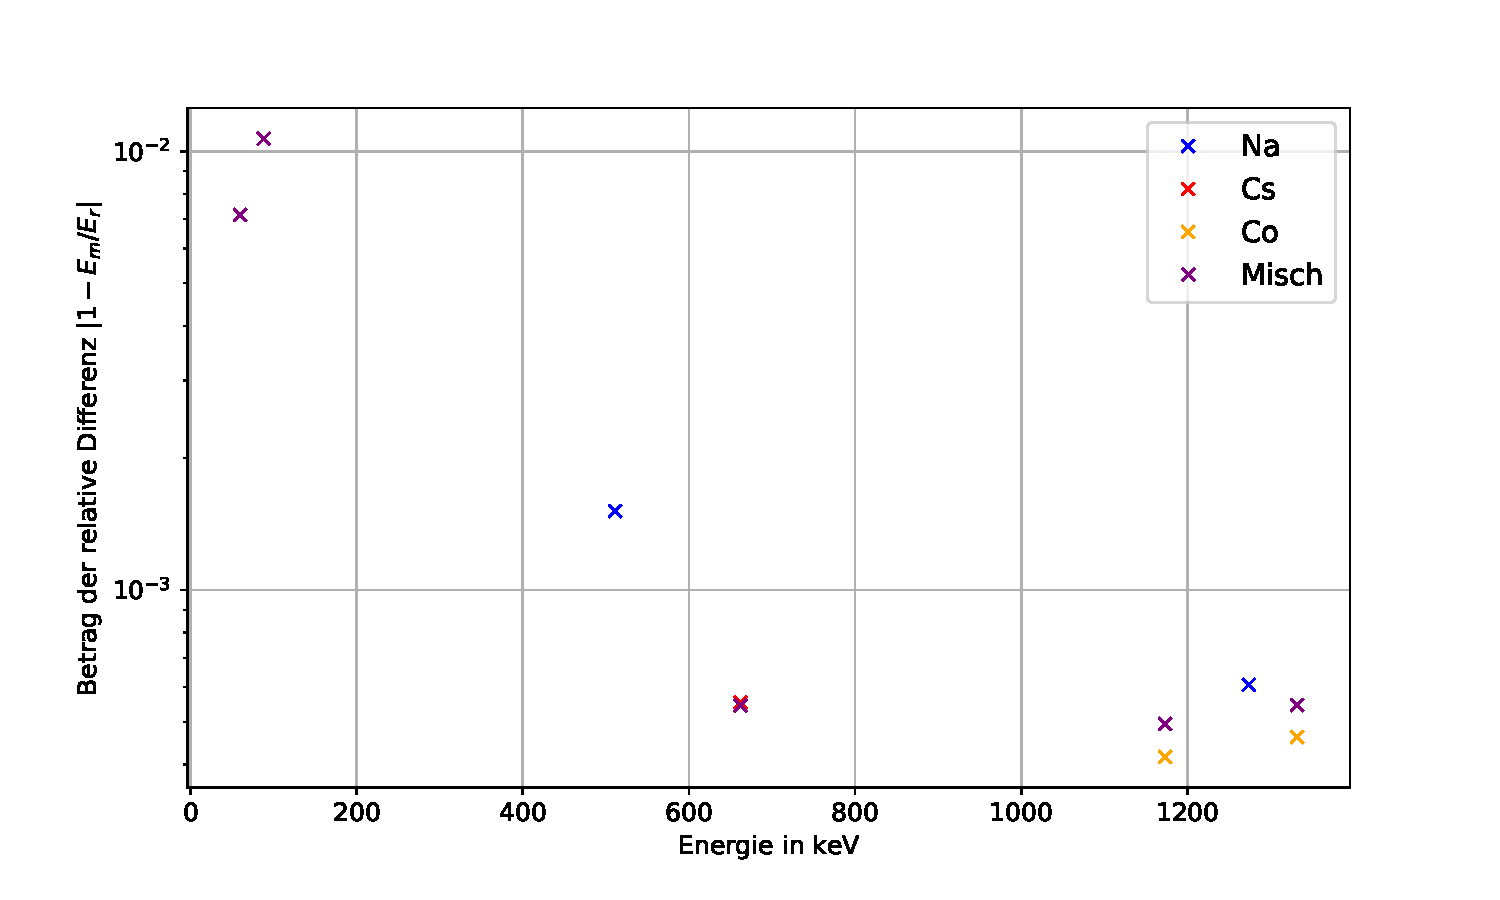
\includegraphics[width= \linewidth]{img/diff_ge_log.pdf}
			\subcaption{
				Betrag der relativen Differenz in logarithmischer Darstellung.
			}
		\end{subfigure}
		\caption{Nichtlinearität des Ge-Detektors.
		Die Unsicherheiten sind nicht abgebildet, da ein Abbilden dieser ein Unterscheiden der Werte unmöglich macht.
		Der Wert Null für die relative Differenz liegt immer im Unsicherheitsintervall.
		}
		\label{fg_diff_ge}
	\end{figure}
\subsection{Energieauflösung und mittlere Ionisationsenergie}
\subsection{Relative Effizienz}
	\subsection{Diskussion}
	% Bezug/Nutzen oder sonst was
	% auch hier die Hypothese wiederholen
	% keine Messwerte hier, nach manchen Menschen, zumindest "direkt" erstellte Diagramme net hier, auch wenn Lesbarkeit-bla
	%TODO Rückstreuungsminimierung durch Deckel abnehmen aber immernoch Luft/Decke/we

	%TODO warum 511 nur bei NA?
	\section{Schlussfolgerung}
	% Rückgriff auf Hypothese und drittes Nennen dieser

	% Quellen zitieren, Websiten mit Zugriffsdatum
	% Verweise auf das Laborbuch (sind erlaubt)
	% Tabelle + Bilder mit Beschriftung
	\printbibliography
\end{document}

%TODO Ich hab der anleitung nen Datum gegeben, weil dass da drauf steht. Vielleicht ist nur das Jahr sinnvoller, weil mans bei veröffentlichungen so machen würde.
